% !TeX program = lualatex
% Archivo principal. Compilar con: lualatex main.tex (dos veces).
\documentclass[11pt,a4paper,oneside]{report}
% Informe de laboratorio de Desarrollo de Videojuegos
% El punto de entrada organizado del informe es main.tex.

% Compilar con LuaLaTeX: fuentes TrueType reales de Windows.
\usepackage{fontspec}
\setmainfont{times.ttf}[Path=C:/Windows/Fonts/,BoldFont=timesbd.ttf,ItalicFont=timesi.ttf,BoldItalicFont=timesbi.ttf]
\setsansfont{times.ttf}[Path=C:/Windows/Fonts/,BoldFont=timesbd.ttf,ItalicFont=timesi.ttf,BoldItalicFont=timesbi.ttf]
\setmonofont{Consolas}[Scale=MatchLowercase]
% Compatibilidad de los enlaces internos con LuaTeX.
\protected\def\pdfinfo{\pdfextension info}
\protected\def\pdfdest{\pdfextension dest}
\protected\def\pdfstartlink{\pdfextension startlink}
\protected\def\pdfendlink{\pdfextension endlink}

\usepackage{graphicx}
\usepackage{xcolor}
\usepackage{array}
\usepackage{float}
\usepackage{tikz}
\usepackage{listings}
\usepackage{tcolorbox}
\tcbuselibrary{listings}
\usetikzlibrary{arrows.meta,positioning,shapes.geometric}

\definecolor{ESPEBlue}{HTML}{18345C}
\definecolor{ESPEGreen}{HTML}{08733F}
\definecolor{ESPEGreenDark}{HTML}{164D35}
\definecolor{PaleGreen}{HTML}{EAF3ED}
\definecolor{AppBlue}{HTML}{345DEE}
\definecolor{PaleBlue}{HTML}{EAF0FF}
\definecolor{SoftGray}{HTML}{F3F5F3}
\definecolor{Ink}{HTML}{243247}
\definecolor{OrangeAI}{HTML}{BC571F}

\setlength{\topmargin}{-0.3in}
\setlength{\oddsidemargin}{-0.1in}
\setlength{\textwidth}{6.3in}
\setlength{\textheight}{9.0in}
\setlength{\headheight}{15pt}
\setlength{\headsep}{0.2in}
\setlength{\footskip}{0.35in}
\setlength{\parskip}{0.45em}
\setlength{\parindent}{1.1em}
\setlength{\emergencystretch}{3em}
\setlength{\tabcolsep}{4.5pt}
\renewcommand{\arraystretch}{1.25}
\renewcommand{\topfraction}{0.92}
\renewcommand{\bottomfraction}{0.78}
\renewcommand{\textfraction}{0.06}
\renewcommand{\floatpagefraction}{0.62}
\setlength{\textfloatsep}{14pt plus 4pt minus 4pt}
\setlength{\floatsep}{14pt plus 4pt minus 4pt}
\pagestyle{headings}
\renewcommand{\chaptername}{Capítulo}
\renewcommand{\contentsname}{Índice general}
\renewcommand{\listfigurename}{Índice de figuras}
\renewcommand{\listtablename}{Índice de tablas}
\renewcommand{\figurename}{Figura}
\renewcommand{\tablename}{\textcolor{ESPEGreen}{Tabla}}
\renewcommand{\appendixname}{Anexo}
\renewcommand{\bibname}{Referencias}
% Tablas: Times New Roman, encabezado en banda verde y reglas sencillas.
\let\originaltabular\tabular
\let\endoriginaltabular\endtabular
\renewenvironment{tabular}[1]{\small\sffamily\color{Ink}\originaltabular{#1}}{\endoriginaltabular}
\newcommand{\thd}[1]{%
  \begingroup
  \setlength{\fboxsep}{3pt}%
  \colorbox{ESPEGreen}{%
    \parbox[t]{\dimexpr\linewidth-2\fboxsep\relax}{%
      \raggedright\sffamily\small\bfseries\color{white}%
      \rule{0pt}{2.6ex}#1\par}%
  }%
  \endgroup
}
\newcolumntype{P}[1]{>{\raggedright\arraybackslash}p{#1}}
\newcommand{\toprule}{\noalign{\vskip 2pt\color{ESPEGreen}\hrule height 1.1pt\vskip 2pt}}
\newcommand{\midrule}{\noalign{\vskip 1pt\color{ESPEGreen!40}\hrule height 0.45pt\vskip 1pt}}
\newcommand{\bottomrule}{\noalign{\vskip 2pt\color{ESPEGreen}\hrule height 1.1pt}}

\newcommand{\url}[1]{\texttt{\detokenize{#1}}}
\pdfinfo{/Title (Tic-Tac-Toe en .NET MAUI - Minimax) /Subject (Informe de laboratorio - Desarrollo de Videojuegos)}

% Enlaces internos del índice con primitivas pdfTeX, sin paquetes externos.
\newcounter{toclinkid}
\makeatletter
\renewcommand{\addcontentsline}[3]{%
  \stepcounter{toclinkid}%
  \edef\@currdest{toclink\arabic{toclinkid}}%
  \pdfdest name{\@currdest} xyz%
  \addtocontents{#1}{\protect\contentsline{#2}{#3}{\thepage}{\@currdest}}%
}
\renewcommand{\contentsline}[4]{%
  \csname l@#1\endcsname%
    {\pdfstartlink attr{/Border [0 0 0]} goto name{#4}%
     \textcolor{ESPEGreen}{#2}\pdfendlink}%
    {\pdfstartlink attr{/Border [0 0 0]} goto name{#4}%
     \textcolor{ESPEGreen}{#3}\pdfendlink}%
}
\makeatother

\setlength{\abovecaptionskip}{5pt}
\setlength{\belowcaptionskip}{3pt}
\makeatletter
\long\def\@makecaption#1#2{%
  \vskip\abovecaptionskip
  {\small\sffamily\centering
   \textcolor{ESPEGreen}{\bfseries #1}\hspace{0.5em}%
   \textcolor{Ink}{#2}\par}%
  \vskip\belowcaptionskip
}
\setlength{\@fptop}{0pt}
\setlength{\@fpbot}{0pt plus 1fil}
\makeatother

\makeatletter
\def\@makechapterhead#1{%
  \vspace*{22pt}%
  {\parindent\z@\raggedright\normalfont
    {\color{ESPEGreen}\sffamily\Large\bfseries\@chapapp\space\thechapter\par}%
    \vskip 8pt%
    {\color{Ink}\sffamily\bfseries\Huge #1\par}%
    \nobreak\vskip 22pt%
  }}
\def\@makeschapterhead#1{%
  \vspace*{22pt}%
  {\parindent\z@\raggedright\normalfont
    {\color{ESPEGreen}\sffamily\bfseries\Huge #1\par}%
    \nobreak\vskip 22pt%
  }}
\renewcommand{\chaptermark}[1]{\markboth{\sffamily\small\color{ESPEGreenDark}\chaptername\space\thechapter.\quad #1}{}}
\renewcommand{\sectionmark}[1]{\markright{\sffamily\small\color{ESPEGreenDark}\thesection\quad #1}}
\renewcommand{\section}{\@startsection{section}{1}{\z@}%
  {-3.4ex\@plus -1ex \@minus -.2ex}%
  {2ex \@plus .2ex}%
  {\normalfont\Large\sffamily\bfseries\color{ESPEGreenDark}}}
\renewcommand{\subsection}{\@startsection{subsection}{2}{\z@}%
  {-2.8ex\@plus -.8ex \@minus -.2ex}%
  {1.4ex \@plus .2ex}%
  {\normalfont\large\sffamily\bfseries\color{ESPEGreenDark}}}
\makeatother

% Dracula / cyberpunk: estilos de código centralizados.
\definecolor{DraculaBG}{HTML}{282A36}
\definecolor{DraculaPanel}{HTML}{21222C}
\definecolor{DraculaFG}{HTML}{F8F8F2}
\definecolor{DraculaPurple}{HTML}{BD93F9}
\definecolor{DraculaCyan}{HTML}{8BE9FD}
\definecolor{DraculaPink}{HTML}{FF79C6}
\definecolor{DraculaGreen}{HTML}{50FA7B}
\definecolor{DraculaComment}{HTML}{A0ACD7}

\lstdefinestyle{draculacyber}{
  language=[Sharp]C,
  basicstyle=\ttfamily\small\color{DraculaFG},
  keywordstyle=\bfseries\color{DraculaPink},
  stringstyle=\color{DraculaGreen},
  commentstyle=\itshape\color{DraculaComment},
  identifierstyle=\color{DraculaFG},
  morekeywords={Minimax,MAX,MIN,si,sino,para,retornar,funcion,profundidad},
  columns=fullflexible,
  keepspaces=true,
  breaklines=true,
  breakatwhitespace=false,
  showstringspaces=false,
  numbers=left,
  numberstyle=\ttfamily\scriptsize\color{DraculaComment},
  numbersep=9pt,
  stepnumber=1,
  frame=none,
  backgroundcolor=\color{DraculaBG},
  xleftmargin=1.8em,
  xrightmargin=0.3em,
  aboveskip=0.5em,
  belowskip=0.5em,
  tabsize=4
}
\lstset{style=draculacyber}

\tcbset{draculacyberbox/.style={
  colback=DraculaBG,
  colframe=DraculaPurple,
  colbacktitle=DraculaPanel,
  coltitle=DraculaCyan,
  boxrule=0.7pt,
  leftrule=2pt,
  arc=1.5mm,
  left=2mm,
  right=2mm,
  top=2mm,
  bottom=2mm,
  before skip=12pt,
  after skip=12pt,
  fonttitle=\bfseries,
  titlerule=0.5pt
}}
\newtcblisting{codigobox}[1]{
  draculacyberbox,
  listing only,
  title={#1},
  listing options={style=draculacyber}
}
\newcommand{\estado}[1]{\textsf{\small #1}}
\newcommand{\ruta}[1]{\texttt{#1}}


\begin{document}
\begin{titlepage}
\thispagestyle{empty}
\centering\sffamily
\vspace*{0.25cm}

\includegraphics[width=0.76\textwidth]{figuras/logo_espe_100.png}\par
\vspace{0.35cm}
{\Large\bfseries UNIVERSIDAD DE LAS FUERZAS ARMADAS -- ESPE\par}
\vspace{0.25cm}
{\large\bfseries DEPARTAMENTO DE CIENCIAS DE LA COMPUTACIÓN\par}
\vspace{0.12cm}
{\large\bfseries CARRERA DE INGENIERÍA EN SOFTWARE\par}
\vspace{0.55cm}
{\Large\bfseries INFORME DE LABORATORIO\par}
\vspace{0.2cm}
{\large\bfseries PROYECTO 8 -- ALTERNATIVA 5\par}
\vspace{0.2cm}
{\LARGE\bfseries TIC-TAC-TOE EN .NET MAUI\par}
\vspace{0.12cm}
{\large\bfseries INTELIGENCIA ARTIFICIAL CON MINIMAX\par}
\vspace{0.55cm}
{\large\bfseries ASIGNATURA: DESARROLLO DE VIDEOJUEGOS\par}
\vspace{0.15cm}
{\large\bfseries UNIDAD 1\par}
\vspace{0.4cm}
{\large\bfseries DOCENTE: ING. CÉSAR VILLACÍS SILVA, MSC.\par}
\vspace{0.45cm}
{\large\bfseries ESTUDIANTES:\par}
\vspace{0.15cm}
\rule{0.58\textwidth}{0.45pt}\par\vspace{0.18cm}
\rule{0.58\textwidth}{0.45pt}\par\vspace{0.18cm}
\rule{0.58\textwidth}{0.45pt}\par
\vspace{0.35cm}
{\large\bfseries GRUPO N.\textsuperscript{o}:\quad\rule{3.5cm}{0.45pt}\par}
\vspace{0.7cm}
{\large\bfseries FECHA: NOVIEMBRE 2026\par}
\end{titlepage}

\pagenumbering{roman}
\chapter*{Resumen}
\addcontentsline{toc}{chapter}{Resumen}
Este informe documenta una aplicación de tres en raya para Android, implementada en C\# con .NET MAUI. La persona juega con \texttt{X}; la computadora responde con \texttt{O} mediante una búsqueda Minimax que recorre las jugadas legales restantes, evalúa victorias, derrotas y empates y favorece ganar pronto o retrasar una derrota. El documento sigue la guía de laboratorio proporcionada para la asignatura: especifica requisitos funcionales y no funcionales, presenta diagramas de casos de uso, secuencia y clases, explica el diseño y describe el trabajo con una adaptación de SRUM+XP.

La revisión se apoya en el código del proyecto MAUI, en la configuración del proyecto, en tres capturas de Visual Studio Community 2026 y en las evidencias existentes del emulador. Estas últimas incluyen 14 imágenes y 25 verificaciones registradas. Los resultados documentan el turno de la IA, el bloqueo de una amenaza, una victoria de la computadora, un empate, el reinicio y la salida. También dejan visible que las opciones de los menús Archivo, Ver y Ayuda aparecen en pantalla pero no ejecutan las acciones anunciadas. El documento separa esos hallazgos de las mejoras propuestas y deja campos editables para los nombres y el grupo de trabajo.

\noindent\textbf{Palabras clave:} videojuegos, .NET MAUI, Android, C\#, Minimax, Tic-Tac-Toe, SRUM, XP.

\tableofcontents
\listoffigures
\listoftables
\clearpage
\pagenumbering{arabic}

\chapter{Introducción y alcance}
\section{Contexto}
La guía de la asignatura propone implementar Tic-Tac-Toe con una inteligencia artificial MinMax y C\# MAUI para móvil, dentro del Proyecto 8, alternativa 5. También solicita carátula, requisitos, diagramas, aplicación de SRUM+XP y métricas de software \cite{guia}. Este trabajo documenta la aplicación ubicada en \ruta{Tic-Tac-Toe/MinMax/C\#\_MAUI\_Mobile}.

El sistema presenta un tablero de 3$\times$3. La persona juega primero y utiliza \texttt{X}; el programa utiliza \texttt{O}. La interfaz se construye con XAML y controles de .NET MAUI. La página maneja el estado del tablero; un controlador independiente calcula la respuesta de la computadora.

Hay una diferencia entre dos materiales de referencia del directorio. La guía DOCX define el formato académico y los entregables. El DOCX denominado \emph{minmax-ia-explicacion} explica una versión Windows Forms, con una clase \texttt{frmTicTacToe}; esa clase no pertenece al proyecto MAUI revisado. Por ello, la explicación de la interfaz de este informe se basa en \texttt{MainPage} y el algoritmo se describe según el controlador Minimax que sí está en el proyecto.

\section{Objetivos}
\subsection{Objetivo general}
Describir el diseño, la implementación y la evidencia disponible de un juego móvil de tres en raya en .NET MAUI cuya computadora selecciona movimientos mediante Minimax.

\subsection{Objetivos específicos}
\begin{enumerate}
  \item Identificar el alcance funcional y las restricciones observables en el código.
  \item Explicar cómo se representa el tablero y cómo se elige una jugada óptima.
  \item Documentar la configuración Android y los pasos para abrir y ejecutar el proyecto desde Visual Studio.
  \item Relacionar las capacidades implementadas con los resultados y límites de la evidencia existente.
  \item Registrar métricas estáticas y proponer trabajo pendiente sin atribuir al proyecto funciones que no implementa.
\end{enumerate}

\section{Alcance del producto}
El alcance implementado es una aplicación Android de una sola pantalla, con tablero, turnos, avisos de fin de partida, botón Nuevo y botón Salir. La plataforma objetivo declarada es \texttt{net10.0-android}; que el proyecto use el modelo de proyecto único de MAUI no significa que el archivo de proyecto actual esté configurado para publicar en iOS, Mac Catalyst o Windows. .NET MAUI permite un proyecto compartido para varias plataformas, pero cada una debe estar incluida como destino de compilación \cite{mauiSingle}.

Quedan fuera del comportamiento implementado el almacenamiento de puntuaciones, la selección de dificultad, la persistencia de partidas, el contenido de ayuda y la ejecución de las opciones internas de los menús. Las etiquetas de esas opciones sí aparecen, pero el código no procesa la selección que devuelve cada hoja de acciones.

\section{Términos y abreviaturas}
\begin{table}[H]
\centering
\small
\caption{Términos y abreviaturas}\label{tab:terms}
\begin{tabular}{P{3.0cm}P{11.5cm}}
\toprule
\thd{Término} & \thd{Definición usada en este informe}\\
\midrule
Estado & Distribución de \texttt{X}, \texttt{O} y casillas vacías en la matriz de 3$\times$3.\\
Nodo & Estado del tablero considerado durante la búsqueda del árbol de jugadas.\\
Jugador MAX & La IA, representada por \texttt{O}, que maximiza la puntuación.\\
Jugador MIN & La persona, representada por \texttt{X}, que minimiza la puntuación de la IA.\\
MAUI & Interfaz de usuario multiplataforma de .NET; el proyecto revisado compila para Android.\\
SRUM+XP & Adaptación solicitada por la guía académica para organizar diseño, desarrollo y pruebas.\\
\bottomrule
\end{tabular}
\end{table}

% ----------------------------------------------------------------------

\chapter{Especificación de requisitos}
\section{Convenciones y base de la especificación}
La guía del curso solicita requisitos según IEEE 830 \cite{guia}. IEEE SA registra IEEE 830-1998 como sustituido por ISO/IEC/IEEE 29148:2011. La edición 2018 de 29148 figura como estándar activo \cite{stand830,stand29148}. Este informe conserva el formato de especificación de la asignatura y no afirma una certificación de conformidad.

Los estados de cumplimiento se interpretan así: \estado{Implementado} indica que el código contiene el comportamiento; \estado{Parcial} indica que se cumple una parte; \estado{Pendiente} indica que el comportamiento solicitado no se encontró en el código revisado. Una captura de pantalla prueba un escenario visible, no todas las entradas posibles.

\section{Requisitos funcionales}
\begin{table}[H]
\centering
\small
\caption{Requisitos funcionales y evidencia asociada}\label{tab:rf}
\begin{tabular}{P{1.0cm}P{7.5cm}P{2.7cm}P{3.0cm}}
\toprule
\thd{ID} & \thd{Requisito} & \thd{Estado} & \thd{Evidencia}\\
\midrule
RF-01 & Al iniciar, mostrar nueve casillas vacías y permitir que la persona empiece con \texttt{X}. & Implementado & \texttt{ResetBoard}; captura 01.\\
RF-02 & Registrar una jugada humana solo si la casilla está vacía y es el turno humano. & Implementado & \texttt{OnCellClicked}; captura 03.\\
RF-03 & Después de una jugada humana válida, calcular y registrar una respuesta de la IA con \texttt{O}. & Implementado & \texttt{AIMove\allowbreak Async}, \texttt{GetBest\allowbreak Move}; captura 02.\\
RF-04 & Detectar victoria de \texttt{X}, victoria de \texttt{O} o empate; mostrar aviso y bloquear jugadas posteriores. & Implementado & \texttt{CheckGameEnd\allowbreak Async}; capturas 08, 09 y 11.\\
RF-05 & Reiniciar la matriz, habilitar las nueve casillas y devolver el turno a la persona. & Implementado & \texttt{OnNewClicked}; captura 10.\\
RF-06 & Cerrar la aplicación desde el control Salir. & Implementado & \texttt{OnExitClicked}; capturas 13 y 14.\\
RF-07 & Mostrar las opciones visibles Archivo, Ver y Ayuda. & Implementado & \texttt{MainPage.xaml}; capturas 04, 05 y 06.\\
RF-08 & Ejecutar la acción elegida en cada menú: Nuevo, Salir, Puntajes, Resetear puntajes, Acerca de y Contenido. & Pendiente & Los manejadores solo muestran la hoja de acciones y descartan su selección.\\
\bottomrule
\end{tabular}
\end{table}

\section{Requisitos no funcionales}
\begin{table}[H]
\centering
\small
\caption{Requisitos no funcionales y observaciones}\label{tab:rnf}
\begin{tabular}{P{1.0cm}P{7.5cm}P{2.7cm}P{3.0cm}}
\toprule
\thd{ID} & \thd{Requisito} & \thd{Estado} & \thd{Nota / límite}\\
\midrule
RNF-01 & La aplicación debe orientarse a Android y declarar una versión mínima de plataforma. & Declarado & \texttt{net10.0-android}; mínimo Android 5.0/API 21 en el proyecto.\\
RNF-02 & El tablero debe conservar proporción cuadrada y adaptarse al ancho disponible. & Implementado & \texttt{OnSizeAllocated}; ancho máximo de 340 unidades MAUI.\\
RNF-03 & Los controles deben ser identificables por automatización y contar con descripción semántica. & Parcialmente implementado & Cada casilla recibe \texttt{AutomationId} y descripción; no hay evidencia de evaluación formal con lector de pantalla.\\
RNF-04 & La jugada de la IA debe responder con rapidez suficiente para un tablero 3$\times$3. & No medido & La búsqueda se ejecuta sincrónicamente y no se guardan tiempos de respuesta.\\
RNF-05 & La lógica del algoritmo debe poder leerse separada de la interfaz. & Implementado & El controlador Minimax es una clase aparte de \texttt{MainPage}.\\
RNF-06 & No se debe aceptar una jugada en una casilla ocupada ni continuar una partida terminada. & Implementado & Validaciones en \texttt{OnCellClicked}; evidencia de ocupación y fin de partida.\\
RNF-07 & La aplicación debe minimizar permisos que no necesita. & Revisar & El manifiesto declara Internet y estado de red; no se encontraron llamadas de red en la lógica revisada.\\
RNF-08 & La interfaz debe usar un idioma uniforme. & Parcial & La interfaz está en español, pero los avisos de victoria y empate están en inglés.\\
\bottomrule
\end{tabular}
\end{table}

\section{Criterios de aceptación}
\begin{enumerate}
  \item Una partida nueva muestra un tablero vacío y empieza el turno humano.
  \item Una casilla ocupada conserva su símbolo cuando se vuelve a pulsar.
  \item Una jugada válida de \texttt{X} va seguida por una respuesta legal de \texttt{O}.
  \item La IA bloquea una amenaza inmediata y, cuando existe una victoria forzada, puede completarla.
  \item El sistema reconoce una partida empatada y bloquea el tablero tras terminar.
  \item Nuevo limpia el estado y Salir cierra el proceso de la aplicación.
  \item Las opciones de menú deben ejecutar sus acciones antes de considerar completo el requisito RF-08.
\end{enumerate}

% ----------------------------------------------------------------------

\chapter{Diseño del sistema}
\section{Arquitectura}
La aplicación utiliza un proyecto MAUI de estilo SDK con interfaz XAML y código C\#. El punto de arranque se configura en \texttt{MauiProgram}; \texttt{App} crea la ventana, \texttt{AppShell} establece la página inicial y \texttt{MainPage} construye y coordina la interfaz del juego. \texttt{UnbeatableAIController} calcula la jugada sin manipular controles visuales.

Las cuatro figuras se generaron con Mermaid. Sus fuentes editables \texttt{01\_arquitectura.mmd}, \texttt{02\_casos\_de\_uso.mmd}, \texttt{03\_secuencia\_turno.mmd} y \texttt{04\_diagrama\_clases.mmd} se incluyen en el directorio \ruta{diagramas\_mermaid}.

\begin{figure}[!htbp]
\centering
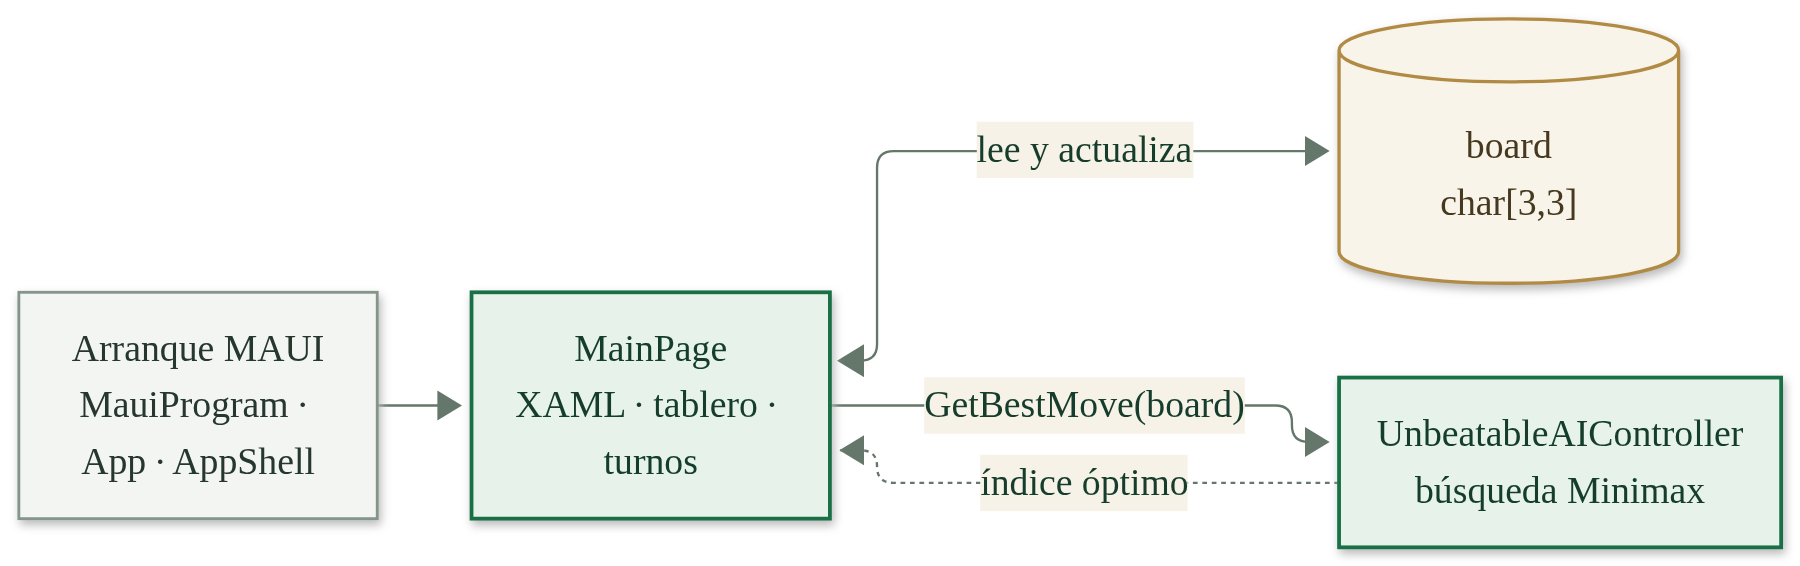
\includegraphics[width=0.92\textwidth,height=0.34\textheight,keepaspectratio]{figuras/diagramas_mermaid/01_arquitectura.png}
\caption[Arquitectura lógica de la aplicación MAUI]{Arquitectura lógica de la aplicación MAUI.}
\label{fig:arquitectura}
\end{figure}

\section{Representación del tablero}
La clase de página mantiene una matriz \texttt{char[3,3]} y un arreglo de nueve botones. Un índice lineal $i$ se convierte a coordenadas usando fila $i/3$ y columna $i\bmod 3$. En XAML la columna se calcula con $i\bmod 3$ y la fila con $i/3$. La matriz y la interfaz se actualizan en el mismo movimiento.

\begin{table}[H]
\centering
\caption{Relación entre índice lineal y coordenadas del tablero}
\label{tab:board-index}
\begin{tabular}{P{2.8cm}P{4.0cm}P{2.5cm}}
\toprule
\thd{Índices} & \thd{Fila de matriz} & \thd{Controles}\\
\midrule
0, 1, 2 & 0 & 1, 2, 3\\
3, 4, 5 & 1 & 4, 5, 6\\
6, 7, 8 & 2 & 7, 8, 9\\
\bottomrule
\end{tabular}
\end{table}

\section{Diagrama de casos de uso}
El actor es una persona que inicia una partida, marca casillas, reinicia, abre los menús o sale. La IA es un servicio interno invocado desde el flujo de una jugada; no es un segundo usuario externo.

\begin{figure}[!htbp]
\centering
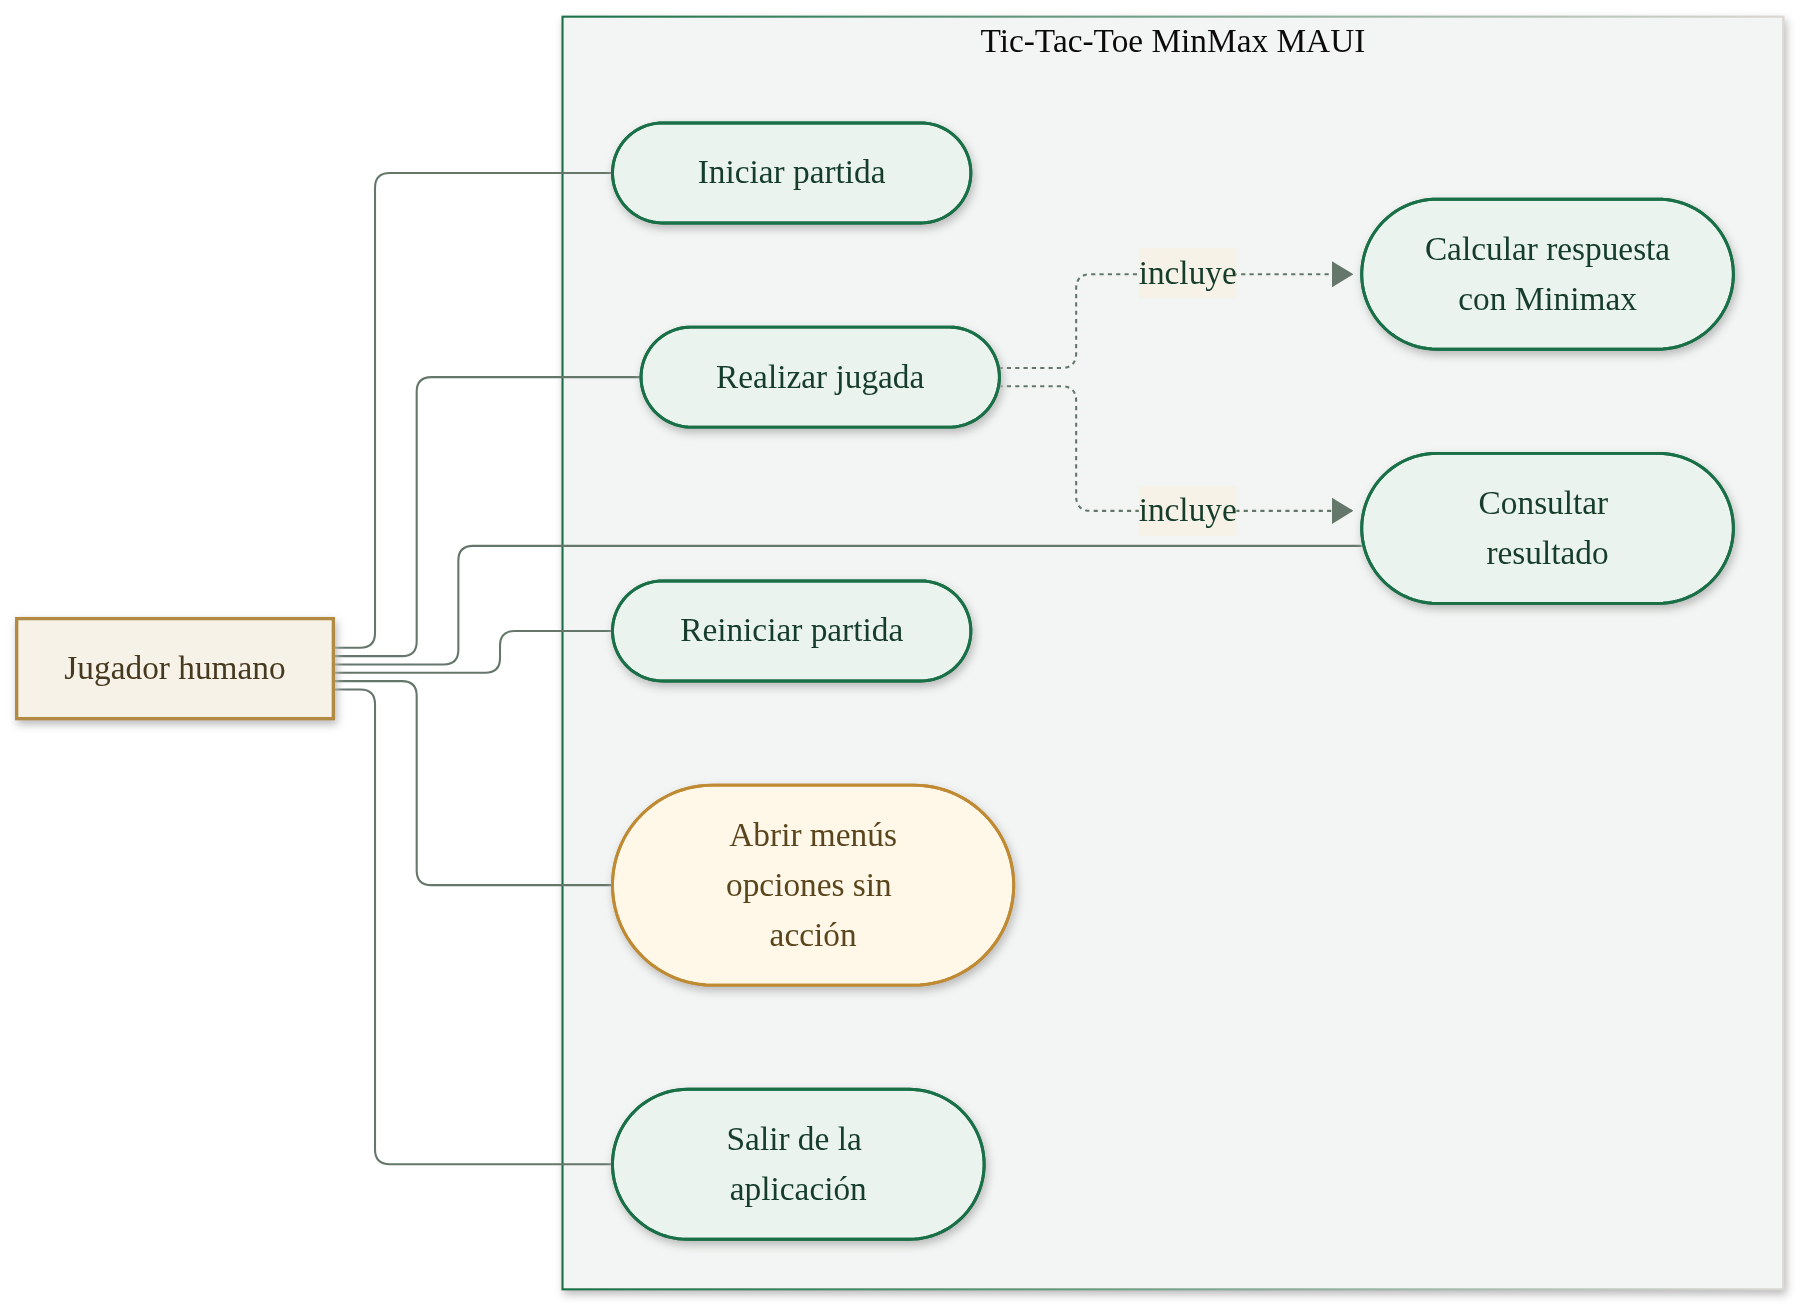
\includegraphics[width=0.96\textwidth,height=0.48\textheight,keepaspectratio]{figuras/diagramas_mermaid/02_casos_de_uso.png}
\caption[Casos de uso de la aplicación]{Casos de uso visibles. La selección de opciones internas de menú está pendiente.}
\label{fig:usecases}
\end{figure}

\subsection{Descripción resumida de casos de uso}
\begin{table}[H]
\centering
\small
\caption{Casos de uso y condición observada}\label{tab:usecases}
\begin{tabular}{P{1.3cm}P{3.1cm}P{8.9cm}}
\toprule
\thd{ID} & \thd{Caso} & \thd{Flujo principal}\\
\midrule
CU-01 & Iniciar partida & La página inicializa el tablero vacío, habilita las casillas y entrega el primer turno a \texttt{X}.\\
CU-02 & Realizar jugada & La persona toca una casilla disponible; el programa escribe \texttt{X}, revisa el fin de partida y solicita la jugada de \texttt{O}.\\
CU-03 & Consultar resultado & Tras cada jugada se buscan líneas ganadoras y se comprueba si el tablero está lleno; si corresponde, se muestra un aviso.\\
CU-04 & Reiniciar & El botón Nuevo borra la matriz y los textos de los botones, los habilita y devuelve el turno a la persona.\\
CU-05 & Abrir menú & Archivo, Ver o Ayuda muestran una hoja de acciones. Elegir una opción no ejecuta una acción en el código actual.\\
CU-06 & Salir & El botón Salir invoca el cierre de la aplicación.\\
\bottomrule
\end{tabular}
\end{table}

\section{Diagrama de secuencia de una jugada}
\begin{figure}[!htbp]
\centering
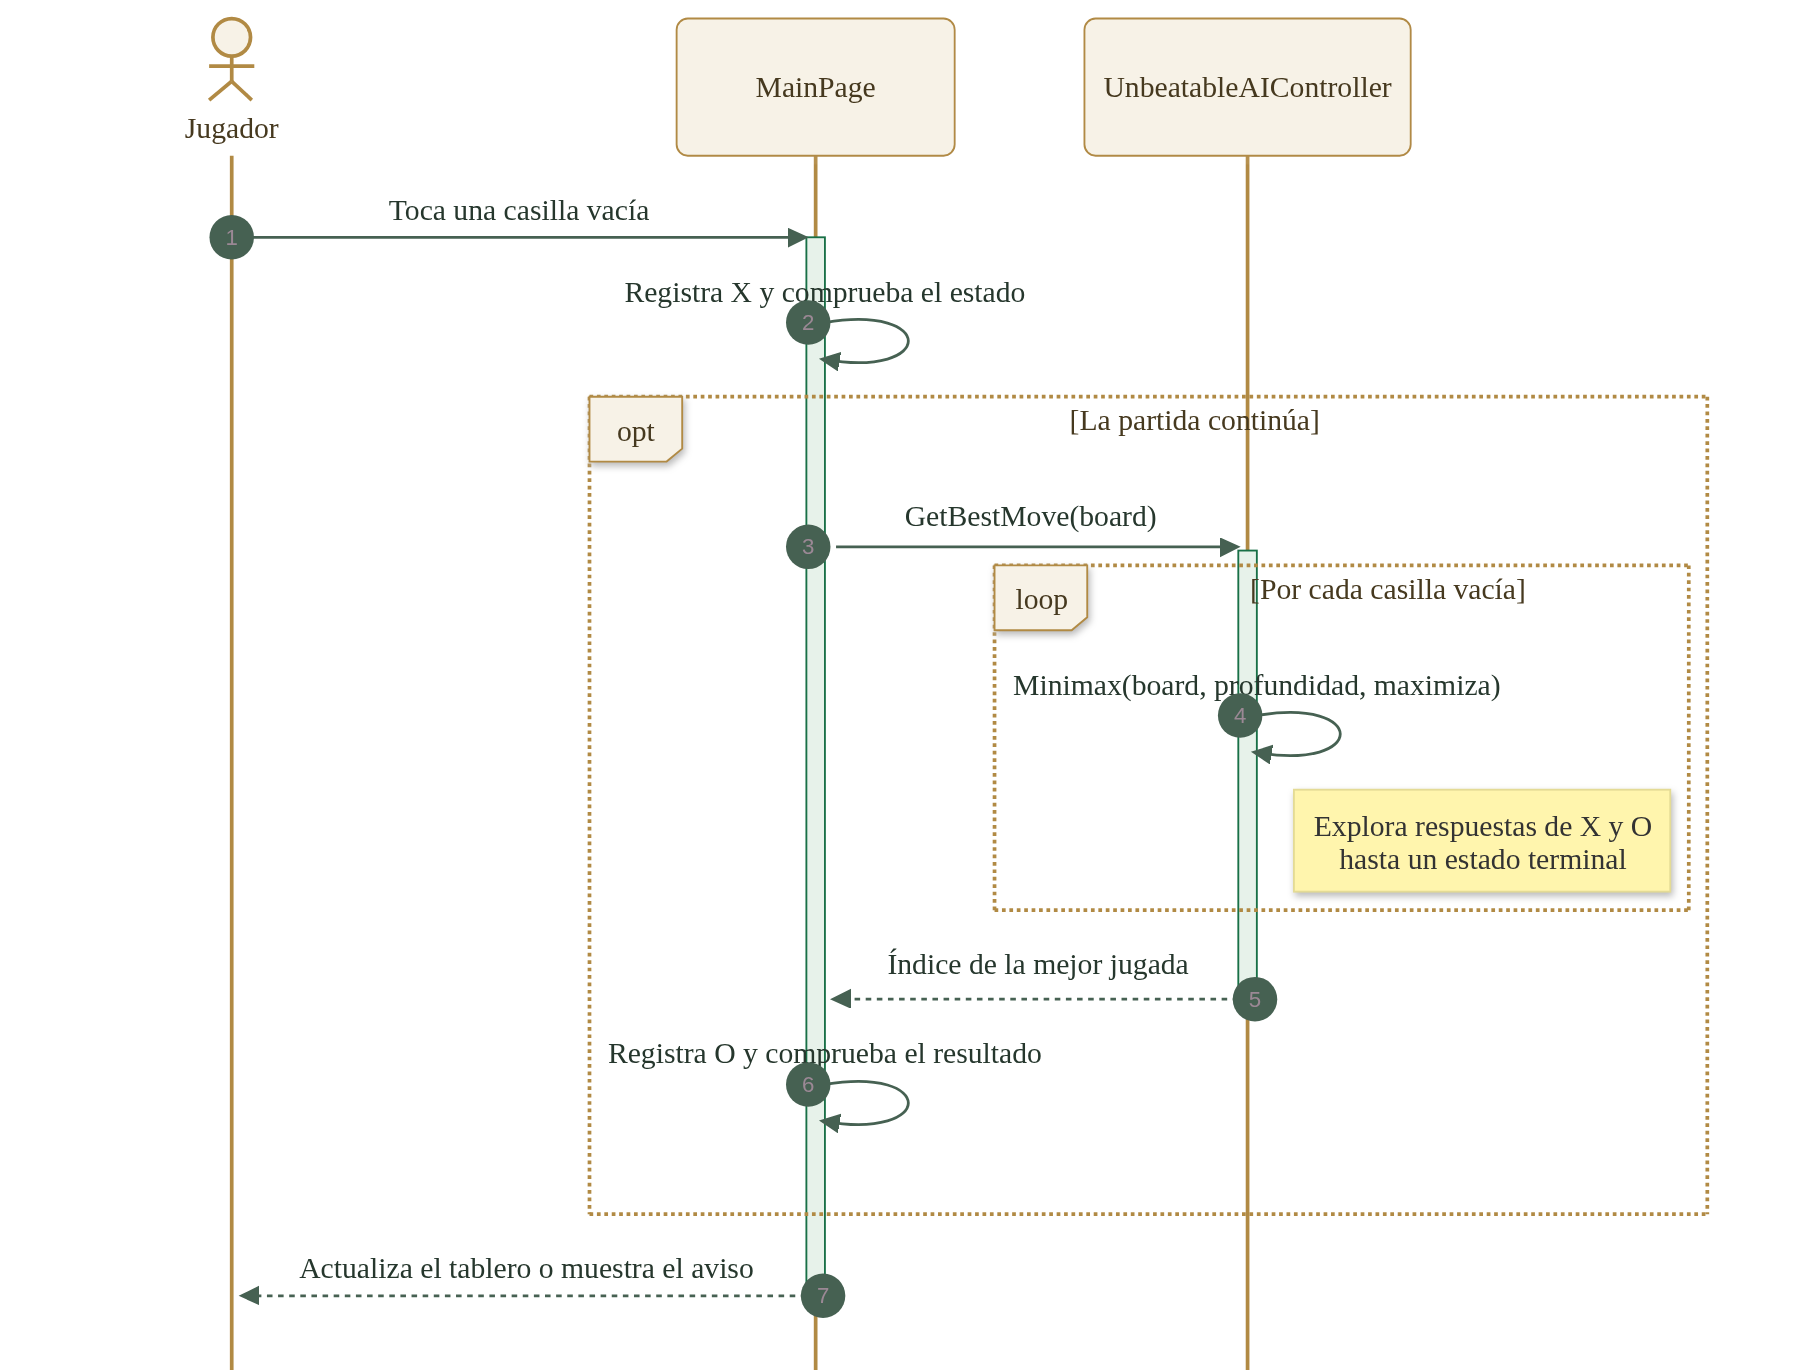
\includegraphics[width=0.92\textwidth,height=0.52\textheight,keepaspectratio]{figuras/diagramas_mermaid/03_secuencia_turno.png}
\caption[Secuencia de una jugada y búsqueda Minimax]{Secuencia de una jugada y búsqueda recursiva de la IA.}
\label{fig:sequence}
\end{figure}

\section{Diagrama de clases}
\begin{figure}[!htbp]
\centering
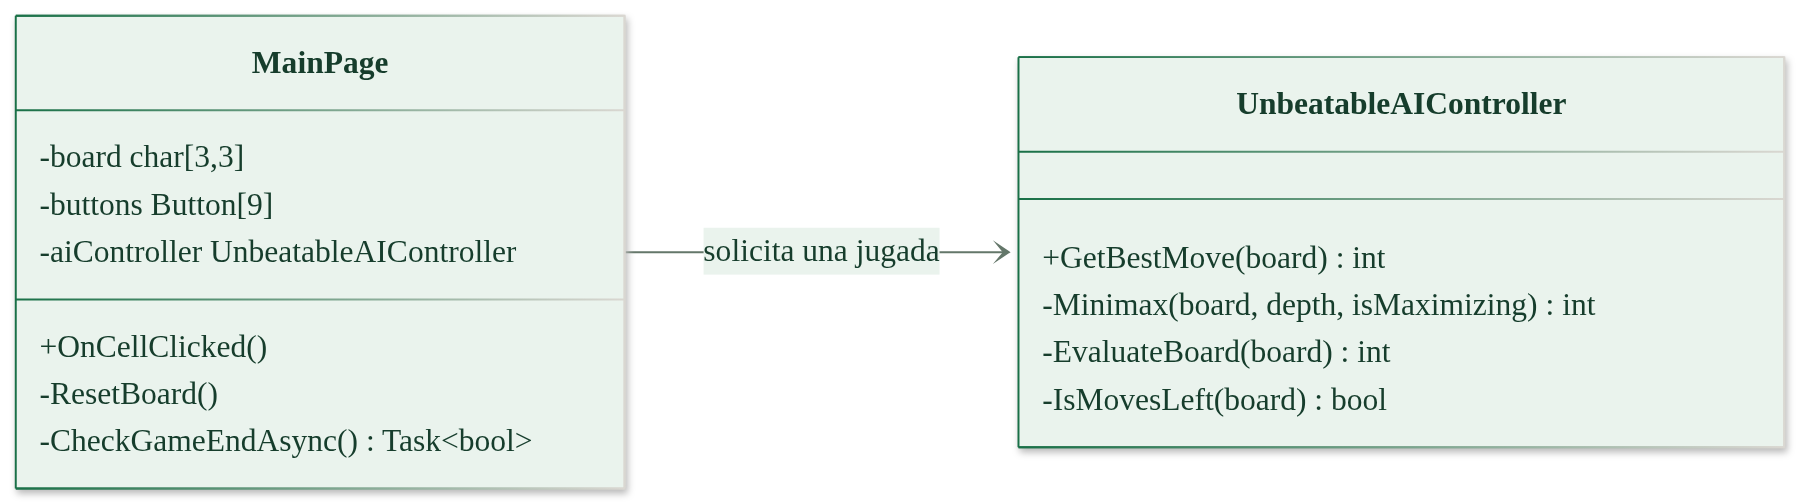
\includegraphics[width=0.98\textwidth,height=0.32\textheight,keepaspectratio]{figuras/diagramas_mermaid/04_diagrama_clases.png}
\caption[Clases centrales de la lógica del juego]{Clases centrales de la lógica del juego y dependencia de Minimax.}
\label{fig:classes}
\end{figure}

% ----------------------------------------------------------------------

\chapter{Algoritmo Minimax}
\section{Idea de decisión}
Minimax es una búsqueda adversarial de suma cero: la IA elige el movimiento que maximiza su resultado y supone que la persona responderá con el movimiento que más lo reduce. El material didáctico de Stanford presenta el mismo principio de búsqueda recursiva sobre árboles de juego \cite{stanfordMinimax}. Para el tablero de tres en raya se exploran jugadas legales hasta alcanzar una victoria, una derrota o un empate.

La puntuación terminal del controlador es:
\[
U(s,d)=
\begin{array}{ll}
10-d, & \mbox{si gana la IA;}\\
-10+d, & \mbox{si gana la persona;}\\
0, & \mbox{si el tablero termina en empate.}
\end{array}
\]
El término $d$ favorece victorias rápidas y retrasa derrotas. En estados no terminales, la rutina no asigna una heurística intermedia: sigue expandiendo los movimientos hasta un resultado terminal.

\section{Procedimiento implementado}
\begin{codigobox}{Pseudocódigo de Minimax}
GetBestMove(board):
    mejorPuntaje = -infinito
    mejorIndice = -1
    para cada indice i entre 0 y 8:
        si board[i] esta vacia:
            colocar O
            puntaje = Minimax(board, profundidad=0, maximiza=false)
            restaurar casilla vacia
            si puntaje > mejorPuntaje:
                guardar puntaje e indice
    devolver mejorIndice

Minimax(board, profundidad, maximiza):
    puntaje = evaluar ganador
    si gana O: devolver 10 - profundidad
    si gana X: devolver -10 + profundidad
    si no quedan movimientos: devolver 0
    si maximiza:
        probar cada casilla vacia como O
        devolver el maximo de las llamadas recursivas
    si no:
        probar cada casilla vacia como X
        devolver el minimo de las llamadas recursivas
\end{codigobox}

\begin{codigobox}{Fragmento C\# del controlador Minimax}
private int Minimax(char[,] board, int depth, bool isMaximizing)
{
    int score = EvaluateBoard(board);
    if (score == 10) return score - depth;
    if (score == -10) return score + depth;
    if (!IsMovesLeft(board)) return 0;
    // Las ramas restantes prueban cada casilla vacia con MAX o MIN.
}
\end{codigobox}

En \texttt{GetBestMove}, cada posible movimiento de \texttt{O} se simula temporalmente en la misma matriz recibida. Después de cada llamada recursiva se restaura el espacio vacío, para que las siguientes alternativas empiecen desde el mismo estado. Como la primera llamada recursiva usa \texttt{isMaximizing=false}, la IA supone que después de su movimiento la persona elegirá la respuesta más perjudicial para ella.

\section{Condiciones terminales y desempate}
\texttt{EvaluateBoard} examina las tres filas, tres columnas y dos diagonales. Devuelve $10$ cuando encuentra una línea de \texttt{O}, $-10$ para una línea de \texttt{X} y $0$ en caso contrario. \texttt{Minimax} distingue entre ese cero no terminal y un empate real mediante \texttt{IsMovesLeft}: solo cuando no quedan casillas devuelve el valor terminal cero.

Si dos movimientos reciben la misma puntuación, el controlador conserva el primero que encuentra porque actualiza la mejor jugada solo cuando \texttt{score > bestScore}. El orden es el índice lineal de 0 a 8. Esto produce desempates deterministas, aunque no prioriza explícitamente centro o esquinas.

\section{Costo de búsqueda}
Sea $b$ el máximo número de movimientos disponibles en un estado y $d$ la profundidad restante. La búsqueda completa tiene costo temporal del orden de $O(b^d)$; aquí $b\leq9$ y $d\leq9$. La recursión es de profundidad acotada y modifica una única matriz de 3$\times$3, por lo que el espacio auxiliar crece con la profundidad, $O(d)$, además del tablero de tamaño fijo. El código no aplica poda alfa-beta ni memorización. Para tres en raya el espacio de búsqueda es pequeño; esta elección mantiene simple la explicación del algoritmo.

La propiedad de no perder se deriva del cálculo óptimo en estados legales y de que ambos resultados terminales se evalúan correctamente. Las capturas existentes demuestran escenarios seleccionados —por ejemplo, bloquear una columna y completar una diagonal—; no sustituyen una enumeración exhaustiva de todos los estados posibles.

% ----------------------------------------------------------------------

\chapter{Desarrollo con SRUM+XP}
\section{Adaptación de la metodología}
La guía del laboratorio solicita SRUM+XP y menciona diseño, desarrollo y pruebas \cite{guia}. El repositorio contiene el código y las evidencias de ejecución, pero no contiene una bitácora de sprints, un tablero histórico, acuerdos de programación en pareja ni registros de integración continua. Por esta razón, la tabla siguiente organiza el trabajo por incrementos comprobables y no atribuye fechas, roles o ceremonias que no están documentados.

\begin{table}[H]
\centering
\small
\caption{Incrementos reconstruidos a partir del proyecto}\label{tab:increments}
\begin{tabular}{P{2.0cm}P{3.2cm}P{5.8cm}P{2.8cm}}
\toprule
\thd{Fase} & \thd{Objetivo} & \thd{Resultado en el código} & \thd{Artefacto}\\
\midrule
Diseño & Separar interfaz, estado y decisión de IA. & Página XAML para presentación; controlador separado para búsqueda. & Diagramas de este informe.\\
Tablero & Construir tablero y turnos. & Matriz 3$\times$3, nueve botones, validación de casilla y reinicio. & \texttt{MainPage.}\allowbreak\texttt{xaml.cs}.\\
Minimax & Integrar decisión adversarial. & Simulación de jugadas y búsqueda Minimax recursiva. & \texttt{UnbeatableAI}\allowbreak\texttt{Controller.cs}.\\
Pruebas & Revisar escenarios en Android. & Automatización por ADB/UIAutomator, capturas PNG y registro JSON. & 14 imágenes, 25 registros.\\
Informe & Entregar requisitos, análisis y resultados. & Especificación, diagramas, configuración y métricas. & Este informe.\\
\bottomrule
\end{tabular}
\end{table}

\section{Prácticas XP observables}
\begin{table}[H]
\centering
\small
\caption{Relación entre prácticas ágiles y evidencia encontrada}\label{tab:xp}
\begin{tabular}{P{3.1cm}P{6.2cm}P{4.5cm}}
\toprule
\thd{Práctica} & \thd{Observación} & \thd{Estado}\\
\midrule
Diseño simple & La búsqueda está aislada en una clase y usa una matriz pequeña, sin dependencias de interfaz. & Evidenciado en el código.\\
Pruebas automatizadas & El script existente consulta la jerarquía UI, toca controles, comprueba el tablero y guarda hashes de imágenes. & Evidencia presente; no se ejecutó durante la elaboración del informe.\\
Retroalimentación frecuente & Los resultados incluyen capturas de cada escenario y un JSON legible por máquina. & Evidencia presente.\\
Programación en pareja & No se encontró registro de sesiones o roles de pareja. & No verificable.\\
Integración continua & No se encontró pipeline ni configuración de compilación automatizada. & No verificado.\\
Refactorización continua & El historial de cambios no está disponible en el directorio de trabajo. & No verificable.\\
\bottomrule
\end{tabular}
\end{table}

\section{Backlog de mejoras priorizado}
\begin{enumerate}
  \item \textbf{Prioridad alta:} conectar el resultado de cada menú con su acción. Nuevo y Salir pueden reutilizar los manejadores existentes; Puntajes requiere definir y almacenar un modelo de puntuación; Ayuda requiere contenido.
  \item \textbf{Prioridad alta:} añadir pruebas unitarias del controlador Minimax para victoria inmediata, bloqueo obligatorio, empate, tablero lleno y ausencia de movimiento.
  \item \textbf{Prioridad media:} unificar el idioma de los avisos y los textos; agregar una presentación accesible del turno y del estado terminal.
  \item \textbf{Prioridad media:} medir el tiempo de decisión en un dispositivo y conservar la medición como evidencia de rendimiento.
  \item \textbf{Prioridad baja:} evaluar poda alfa-beta o memorización si el tablero se generaliza a juegos con mayor espacio de búsqueda.
\end{enumerate}

% ----------------------------------------------------------------------

\chapter{Implementación y configuración en Visual Studio}
\section{Estructura del proyecto}
\begin{table}[H]
\centering
\caption{Archivos de entrada más relevantes}
\label{tab:files}
\begin{tabular}{P{4.8cm}P{10.0cm}}
\toprule
\thd{Archivo} & \thd{Responsabilidad observada}\\
\midrule
\texttt{TicTacToeMinMax\allowbreak.csproj} & Destino Android, identidad de aplicación, recursos e inclusiones de paquetes.\\
\texttt{MauiProgram.cs} & Construye la aplicación MAUI y agrega registro de depuración en configuración DEBUG.\\
\texttt{App.xaml.cs} & Crea la ventana principal con \texttt{AppShell}.\\
\texttt{AppShell.xaml} & Declara \texttt{MainPage} como contenido inicial.\\
\texttt{MainPage.xaml} & Define textos, tablero contenedor, botones, menús y estilos.\\
\texttt{MainPage.xaml.cs} & Coordina turnos, estado, eventos, reinicio, salida y resultados.\\
\texttt{UnbeatableAI}\allowbreak\texttt{Controller.cs} & Evalúa estados y busca el movimiento de \texttt{O}.\\
\texttt{AndroidManifest.xml} & Manifiesto y permisos Android declarados.\\
\texttt{launchSettings.json} & Incluye un perfil llamado \emph{Windows Machine}; no identifica el emulador Android.\\
\bottomrule
\end{tabular}
\end{table}

\section{Configuración comprobada}
La inspección del equipo y del proyecto encontró Visual Studio Community 2026 versión 18.11.0, SDK de .NET 10.0.402 y las cargas de trabajo de MAUI/Android 10.0.110. El proyecto usa MAUI con destino Android y mínimo de plataforma API 21. En la barra de Visual Studio se ve la configuración \emph{Debug}, \emph{Any CPU} y el destino seleccionado \emph{Pixel 7 -- API 36.0 (Android 16.0 -- API 36)}. Los requisitos de plataforma de MAUI para Android 5.0/API 21 o posterior coinciden con el valor mínimo del proyecto \cite{mauiPlatforms}.

\begin{table}[H]
\centering
\caption{Propiedades del proyecto y valores encontrados}
\label{tab:config}
\begin{tabular}{P{5.0cm}P{9.8cm}}
\toprule
\thd{Propiedad} & \thd{Valor observado}\\
\midrule
Target framework & \texttt{net10.0-android}\\
Tipo de salida & \texttt{Exe}\\
MAUI y proyecto único & \texttt{UseMaui=true}; \texttt{SingleProject=true}\\
Nullable reference types & Habilitado\\
Versión mínima Android & \texttt{SupportedOSPlatformVersion=21.0}\\
Título de aplicación & \texttt{Tic-Tac-Toe}\\
Application ID & \texttt{com.companyname.tictactoeminmax}\\
Versión de aplicación & \texttt{1.0}; versión numérica \texttt{1}\\
Icono e imagen de inicio & \texttt{Resources/AppIcon/appicon.png}; pantalla inicial blanca, base 128$\times$128\\
Imagen incluida & \texttt{Resources/Images/pic\_character.png}\\
Paquetes & \texttt{Microsoft.Maui.Controls} con \texttt{\$(MauiVersion)} y \texttt{Microsoft.Extensions.Logging.Debug} 10.0.0\\
\bottomrule
\end{tabular}
\end{table}

El proyecto incluye una sola plataforma en \texttt{TargetFramework}, aunque MAUI permita compartir código con otros destinos. El emulador seleccionado en Visual Studio es evidencia de configuración de depuración; no se interpreta como una ejecución nueva de la aplicación. El README de las capturas identifica el dispositivo usado para la evidencia anterior como \texttt{emulator-5554}; no se atribuye un número de serie a la selección mostrada por Visual Studio.

\section{Capturas de configuración en Visual Studio}
Las capturas se generaron desde la ventana de Visual Studio con el proyecto MAUI cargado. Se muestran el destino Android seleccionado y la configuración del archivo de proyecto; no se modificó el código para producirlas.

\begin{figure}[!htbp]
\centering
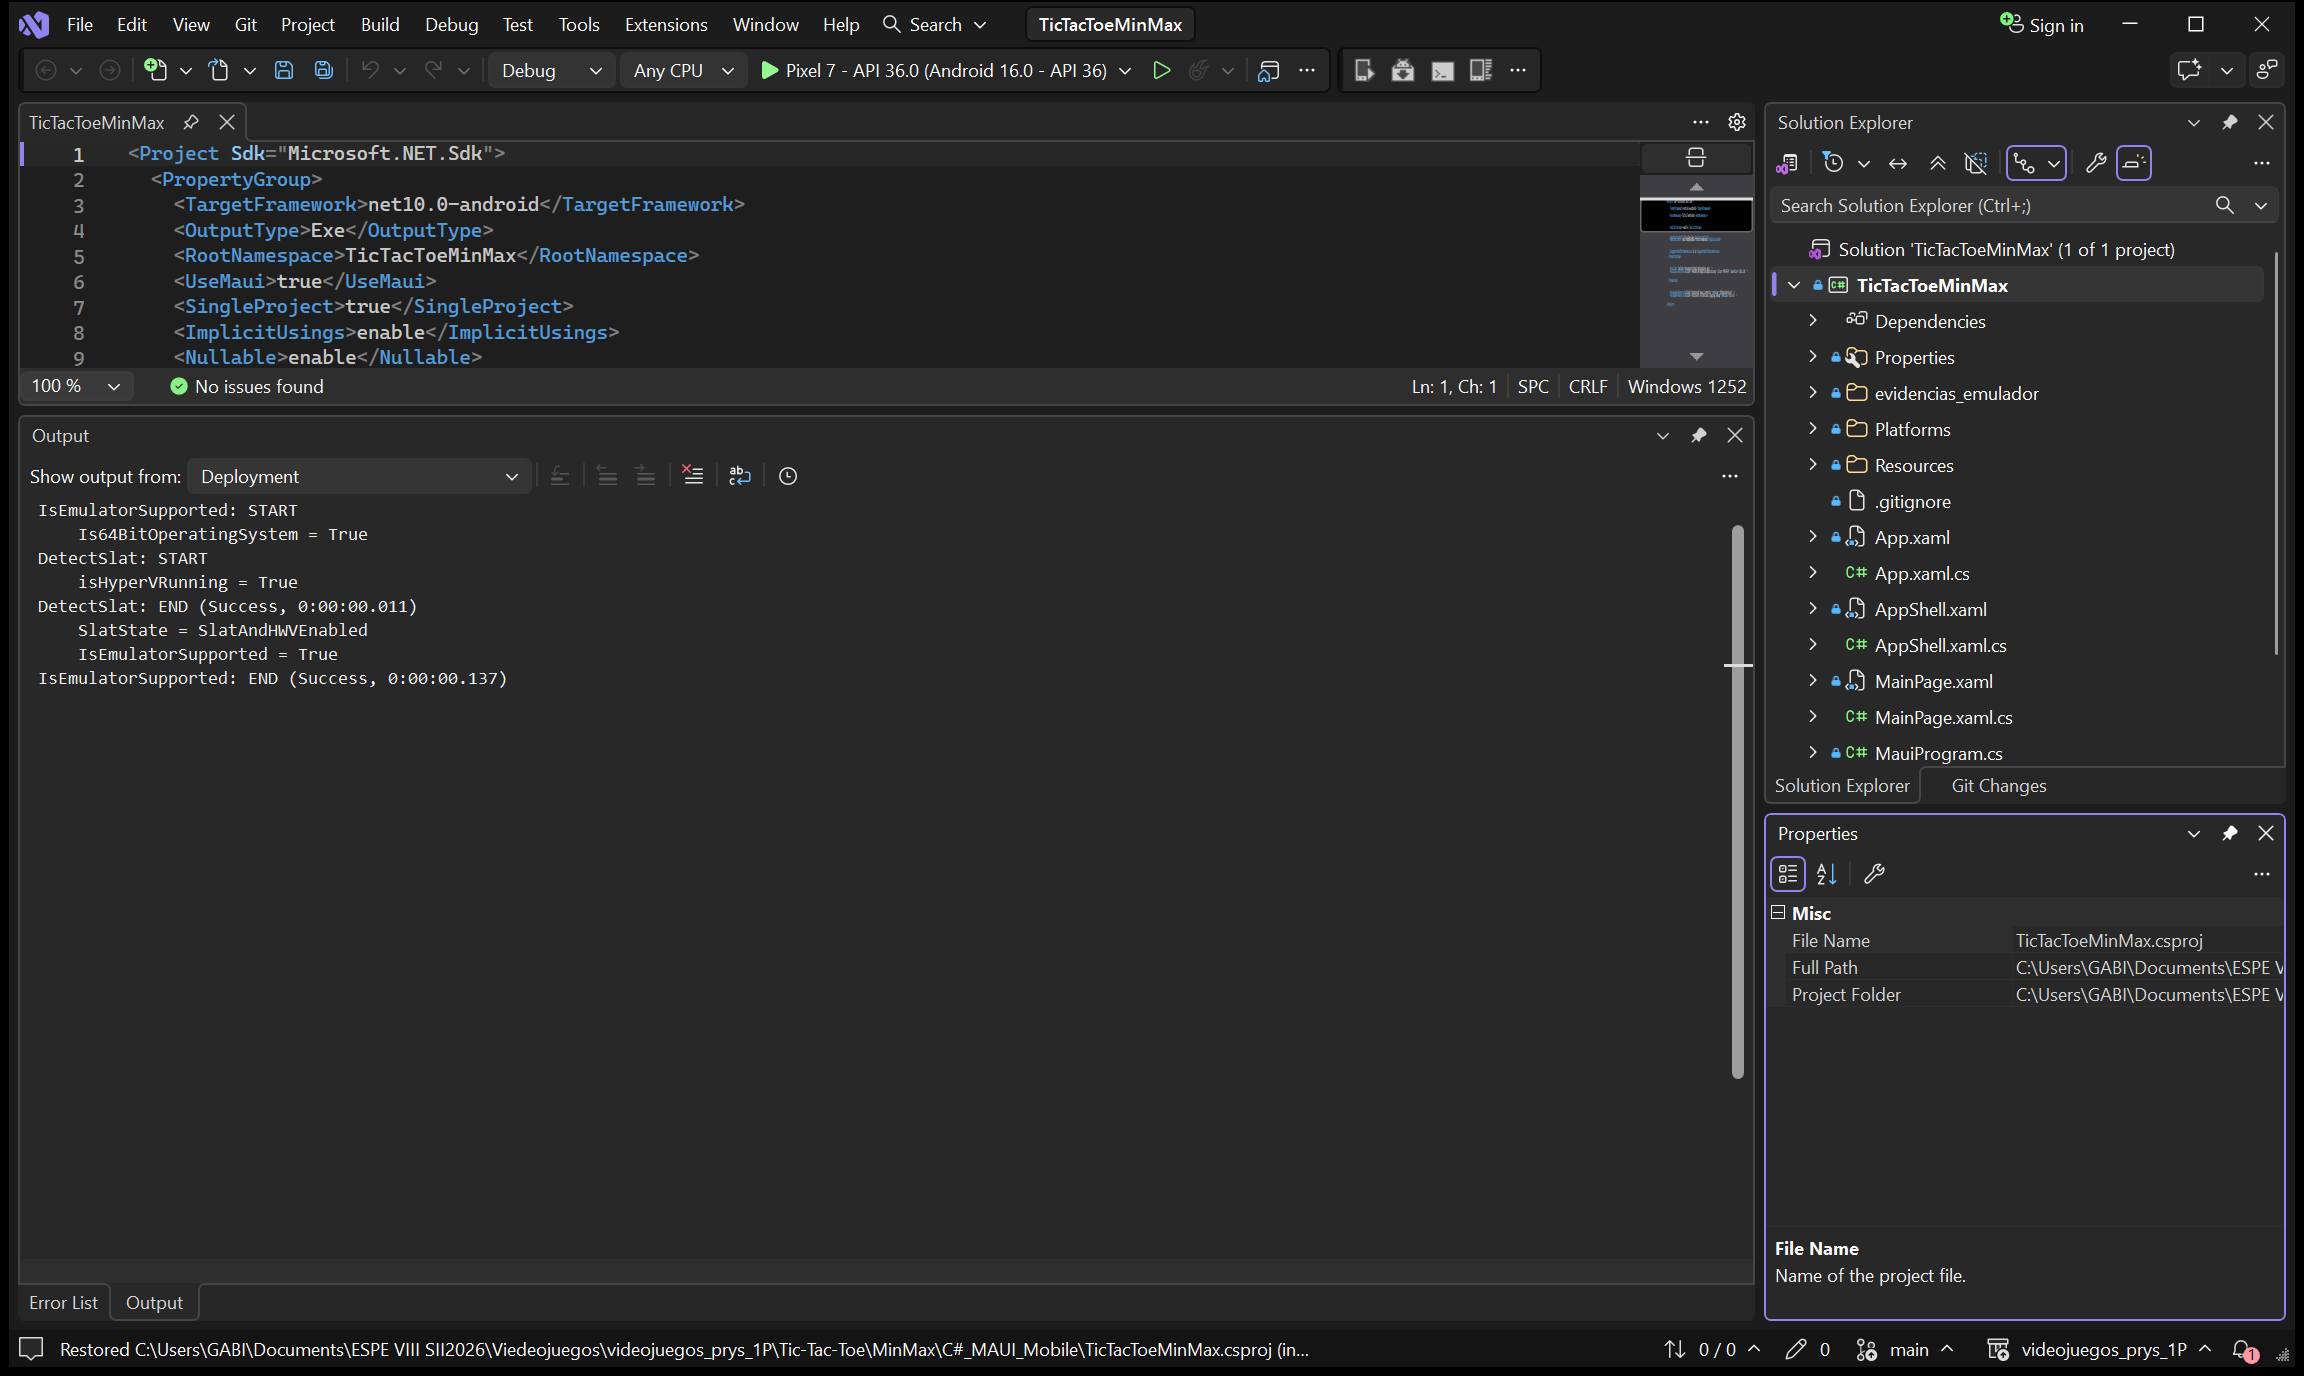
\includegraphics[width=\textwidth]{configuraciones_visual_studio/01_visual_studio_proyecto.png}
\caption{Visual Studio Community 2026 con el proyecto cargado. La barra muestra Debug, Any CPU y el emulador Android seleccionado; el editor muestra el destino \texttt{net10.0-android}.}
\label{fig:vs-project}
\end{figure}

\begin{figure}[!htbp]
\centering
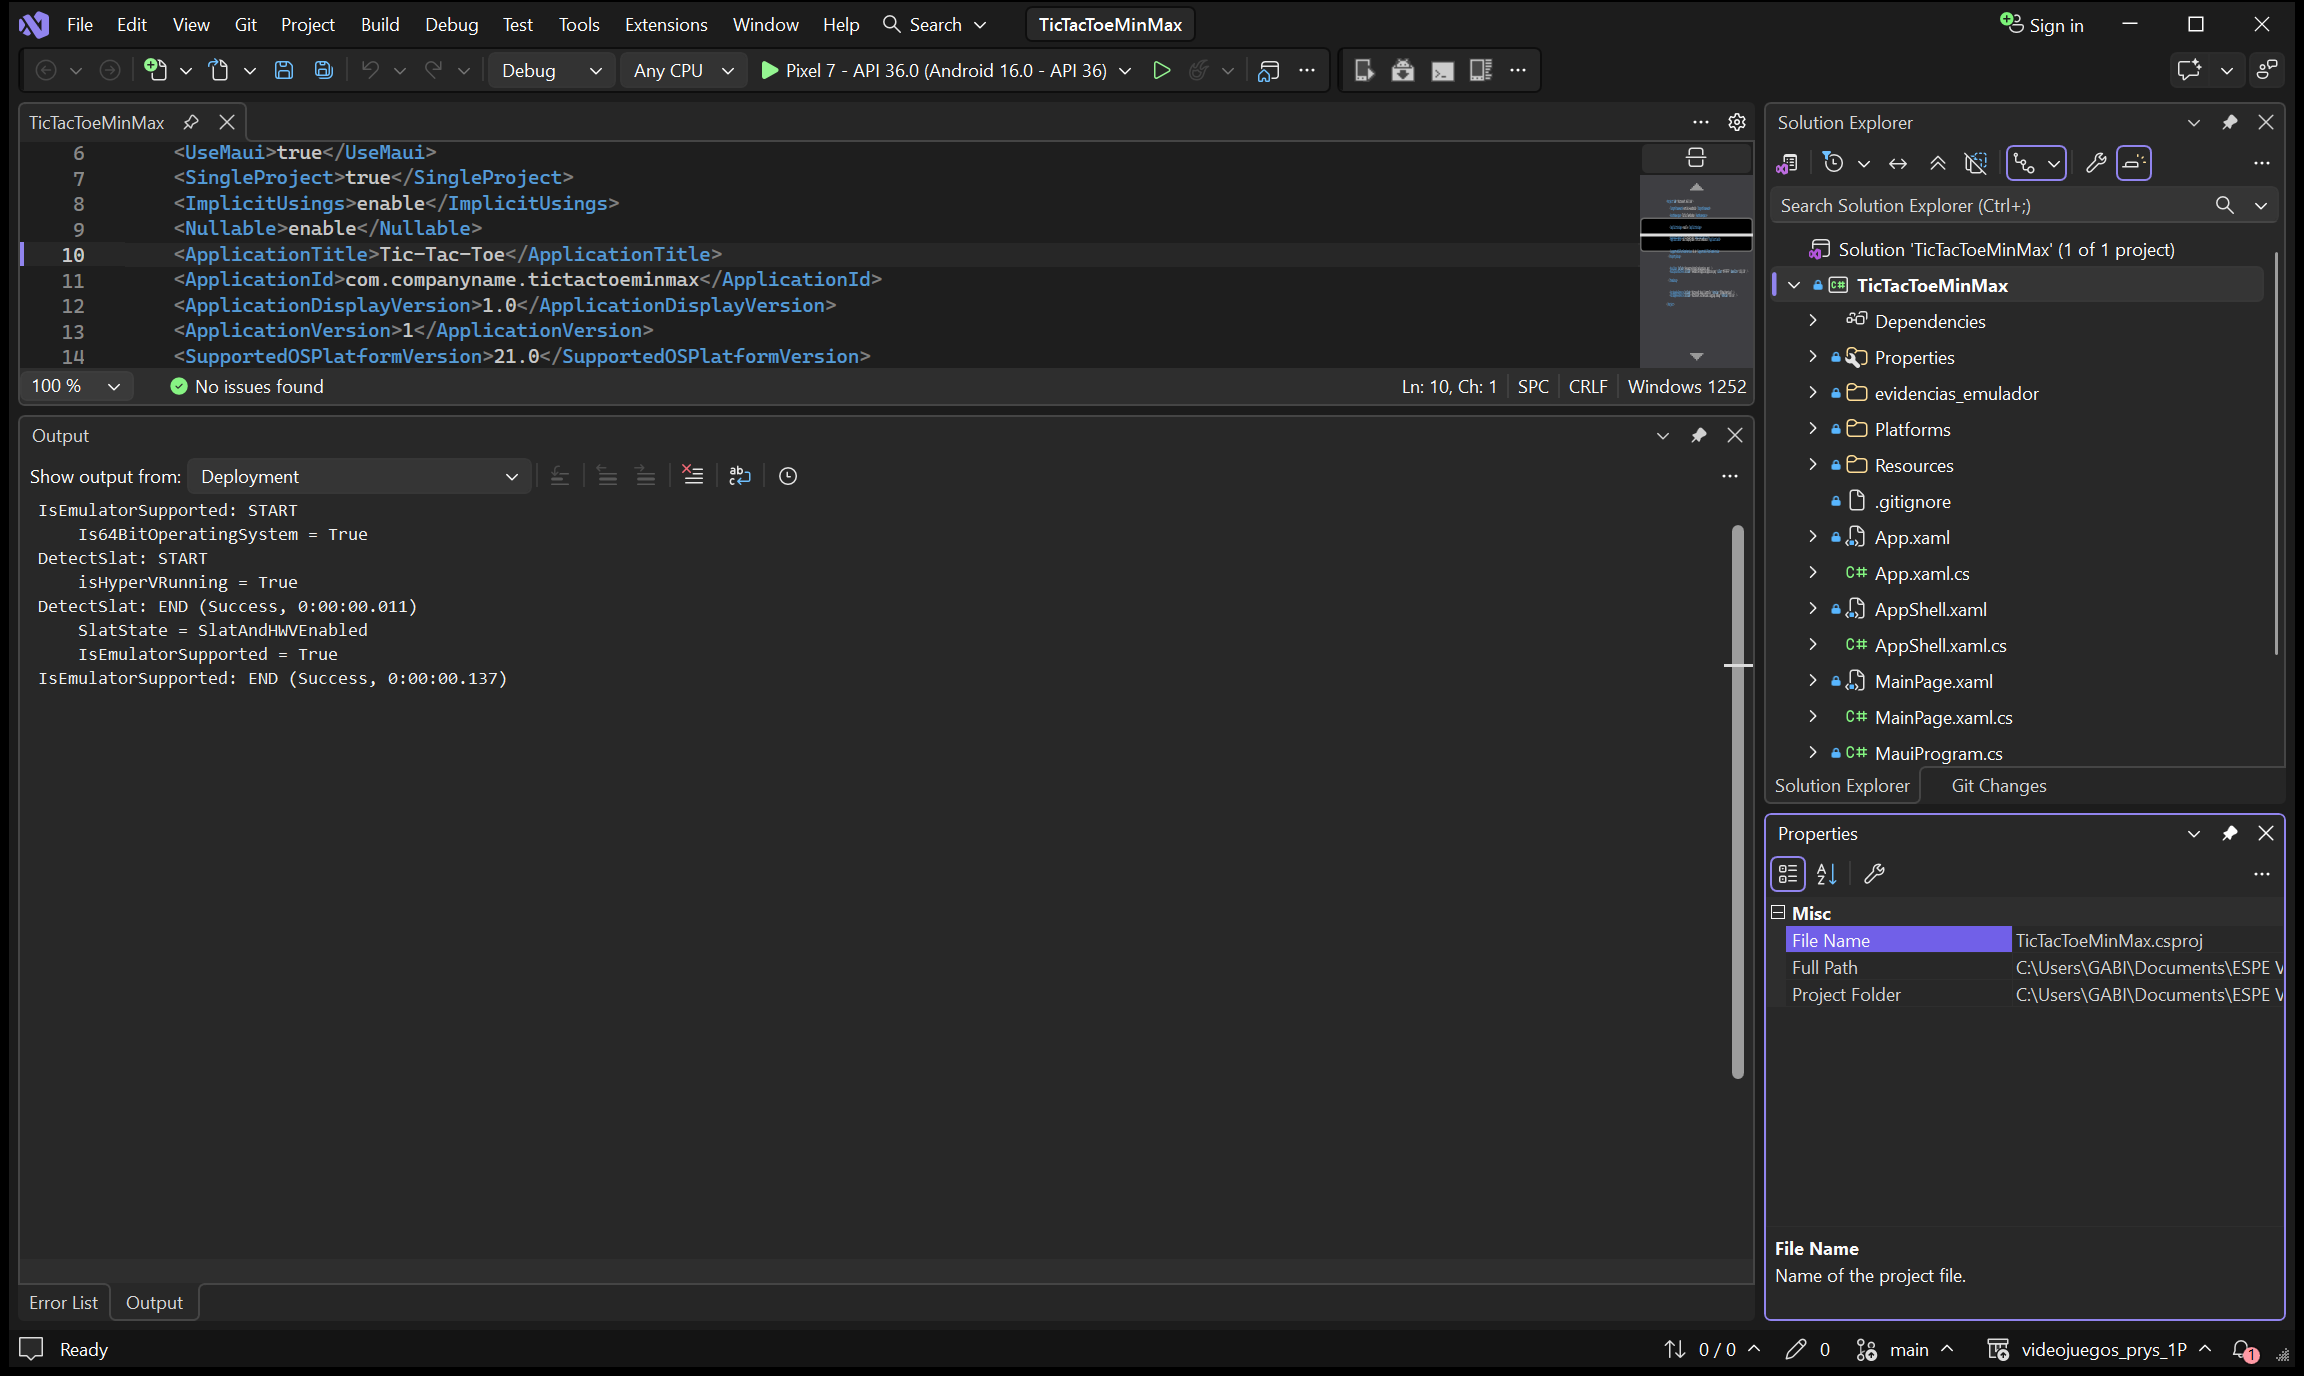
\includegraphics[width=\textwidth]{configuraciones_visual_studio/02_visual_studio_target_android.png}
\caption{Configuración de aplicación y plataforma en el \texttt{.csproj}: título, Application ID, versiones y mínimo Android API 21.}
\label{fig:vs-target}
\end{figure}

\begin{figure}[!htbp]
\centering
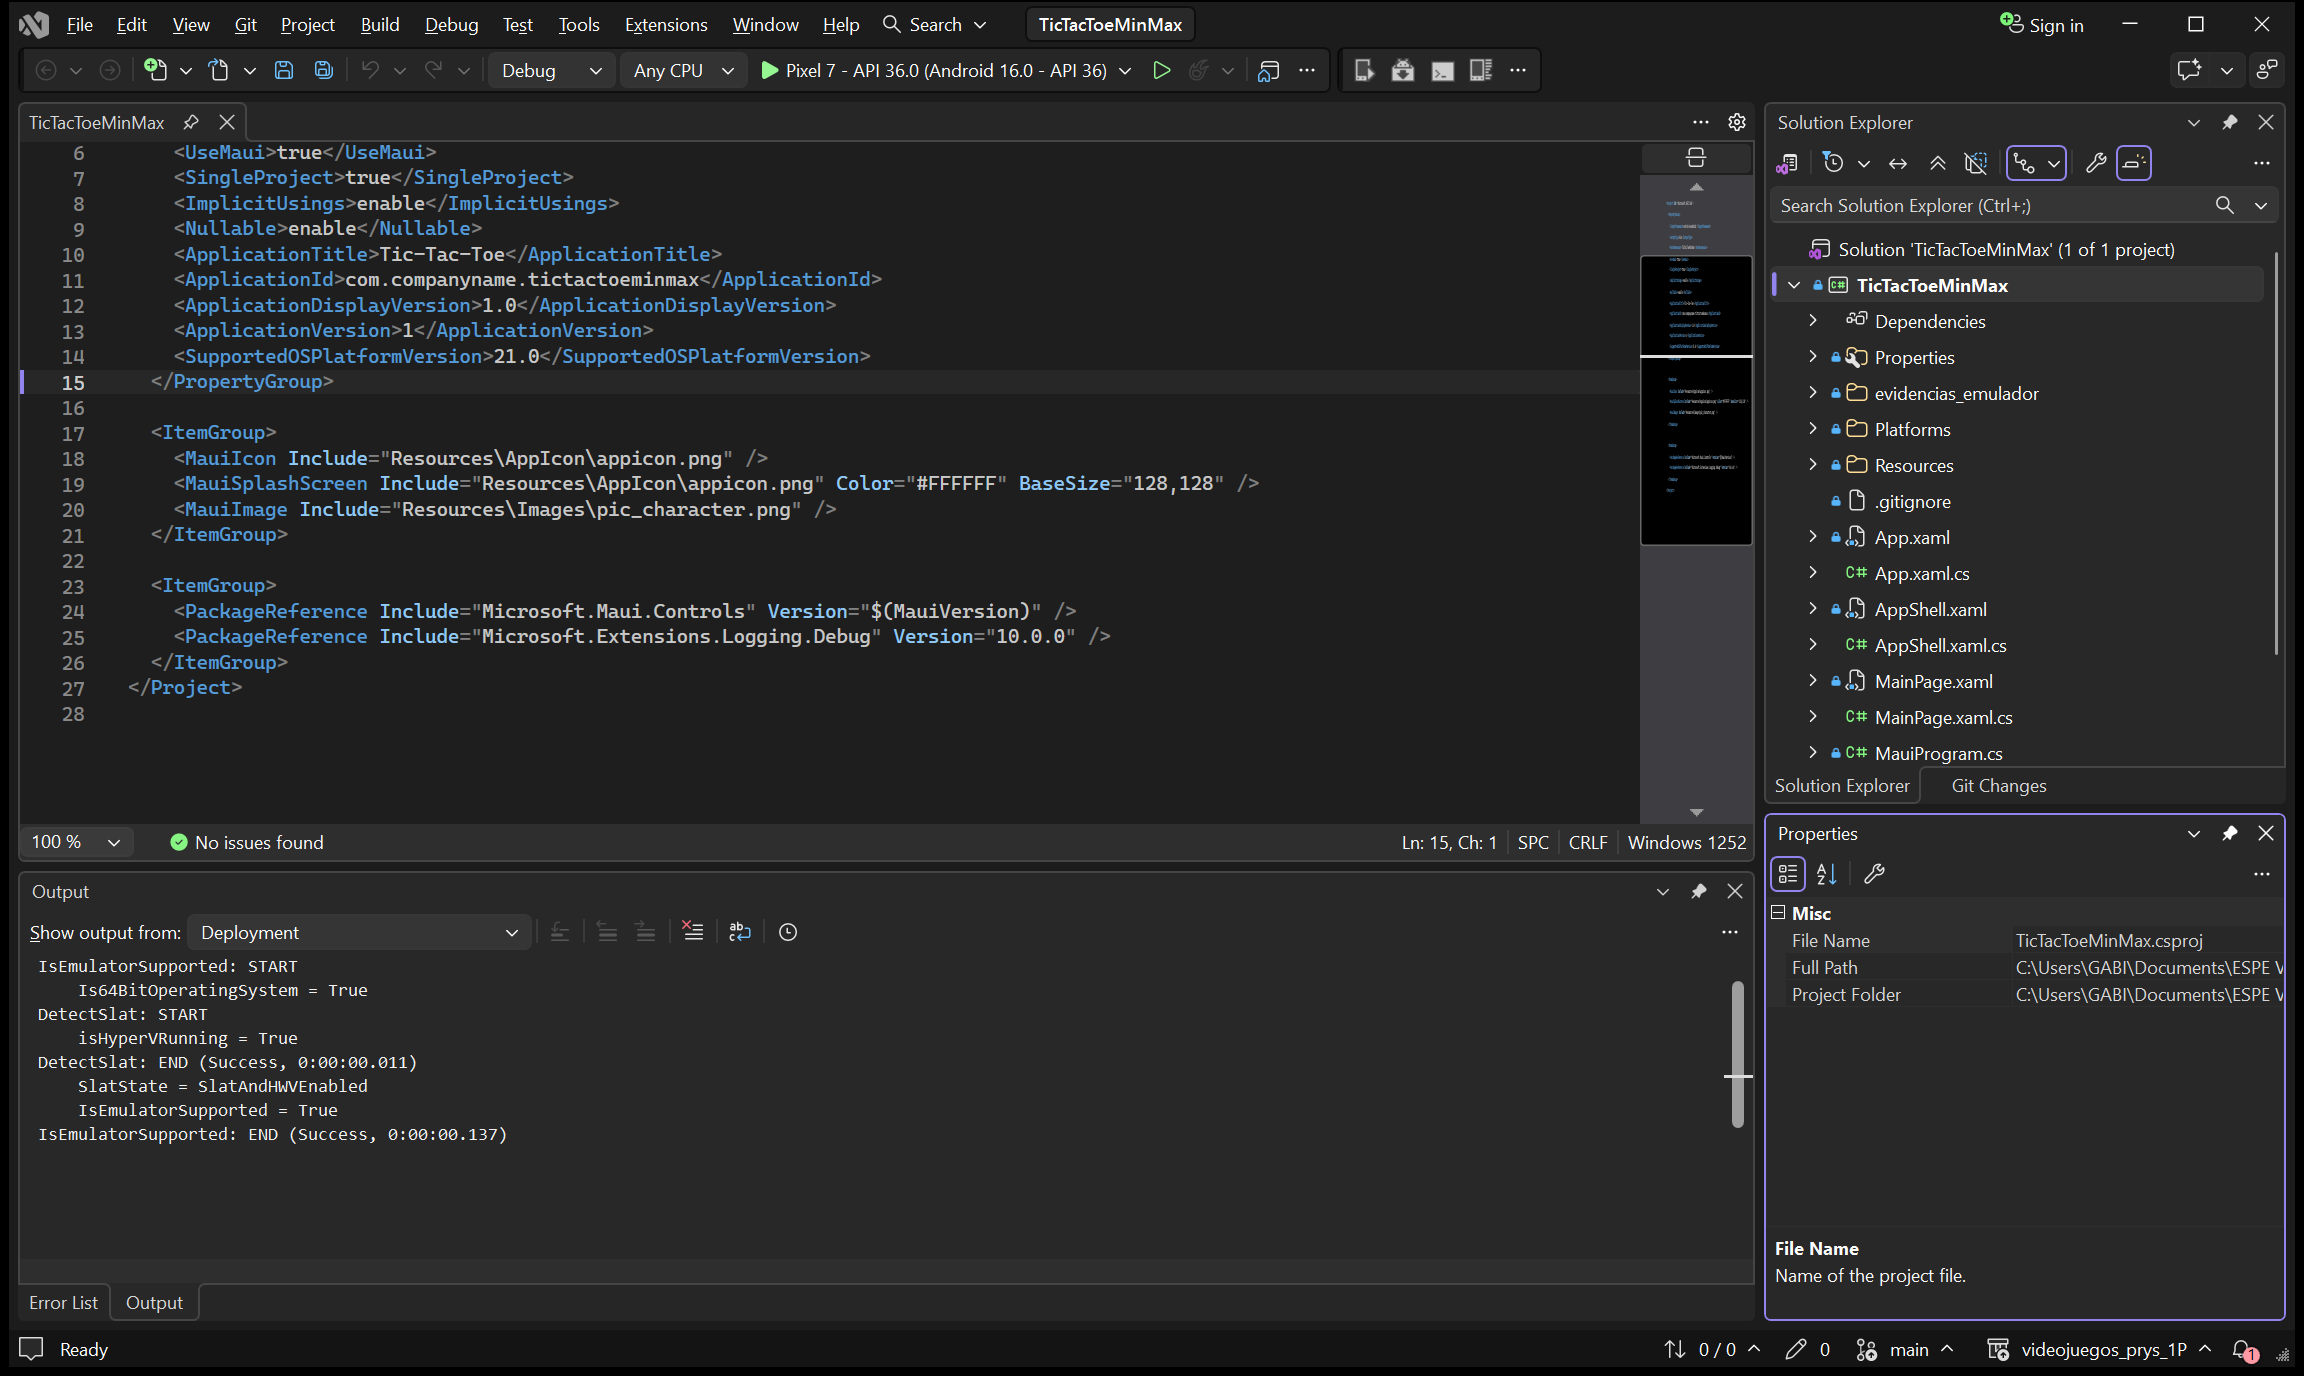
\includegraphics[width=\textwidth]{configuraciones_visual_studio/03_visual_studio_paquetes_recursos.png}
\caption{Recursos MAUI y referencias de paquetes declarados en el proyecto.}
\label{fig:vs-resources}
\end{figure}

\section{Pasos para abrir y ejecutar desde Visual Studio}
\begin{enumerate}
  \item Iniciar Visual Studio y escoger \textbf{Abrir un proyecto o una solución}.
  \item Seleccionar \ruta{TicTacToeMinMax.csproj} dentro de \ruta{Tic-Tac-Toe/MinMax/C\#\_MAUI\_Mobile}. El directorio no contiene un archivo de solución para este proyecto MAUI; se abre directamente el proyecto.
  \item Esperar la restauración de paquetes. Para desarrollar MAUI en Windows deben estar instalados el SDK de .NET MAUI y los componentes Android; Microsoft documenta su instalación desde Visual Studio Installer y la verificación mediante las cargas de trabajo instaladas \cite{mauiInstall}.
  \item En la barra de depuración, seleccionar \textbf{Debug}, \textbf{Any CPU} y un emulador Android. La captura de este equipo muestra \textbf{Pixel 7 -- API 36.0 (Android 16.0 -- API 36)}.
  \item Usar \textbf{Iniciar} o presionar \textbf{F5}. Si Visual Studio solicita un dispositivo, elegir un emulador Android disponible y esperar el despliegue.
  \item En la aplicación, tocar una casilla vacía. Comprobar que la persona juega con \texttt{X} y que la respuesta de Minimax aparece con \texttt{O}.
  \item Usar Nuevo para limpiar el tablero. La opción Salir cierra la aplicación; las opciones de los menús Archivo, Ver y Ayuda son solo presentacionales en la versión revisada.
\end{enumerate}

\section{Configuración Android que conviene conservar}
Las cargas de trabajo y el destino Android son coherentes con el archivo del proyecto. El perfil de \texttt{launchSettings.json} llamado \emph{Windows Machine} no describe el dispositivo Android; la selección del emulador se realiza desde la barra de depuración de Visual Studio. El manifiesto declara \texttt{INTERNET} y \texttt{ACCESS\_NETWORK\_STATE}; al no encontrarse uso de red en la lógica del juego, conviene justificar o retirar esos permisos en una revisión de configuración.

% ----------------------------------------------------------------------

\chapter{Validación y métricas}
\section{Evidencia de ejecución existente}
La carpeta \ruta{evidencias\_emulador/capturas\_20261104\_175826} conserva 14 capturas PNG, un README, un archivo \texttt{resultados.json} con hashes SHA-256 y un script de automatización basado en ADB y UIAutomator. El README registra 25 verificaciones con estado PASS. La revisión del JSON y del README muestra que ese estado debe leerse junto con el detalle de cada caso: en las opciones internas de menú, PASS significa que la selección no alteró la partida, porque el menú carece de manejadores, no que la opción anunciada funcione.

La evidencia incluye el inicio, turno humano e IA, selección de casilla ocupada, menús, bloqueo de una amenaza, victoria de la IA, bloqueo tras finalizar, reinicio, empate, salida y reapertura. El script evita crear una victoria humana artificial: la propia IA bloquea las jugadas ganadoras de \texttt{X}. Por eso el paquete de evidencia no contiene una captura de victoria humana. Este comportamiento es coherente con la finalidad de Minimax, pero no reemplaza una prueba unitaria de todos los estados.

El registro identifica \texttt{02\_turno\_humano\_ia.png} y \texttt{03\_casilla\_ocupada.png} con el mismo hash. La segunda captura documenta el paso de prueba pero su imagen es idéntica a la anterior; debe contarse como una limitación de la evidencia visual. Este informe conserva ambas con sus nombres originales para mantener correspondencia con el JSON.

\begin{table}[H]
\centering
\caption{Resumen de escenarios de aceptación documentados}
\label{tab:tests}
\begin{tabular}{P{4.0cm}P{2.0cm}P{8.5cm}}
\toprule
\thd{Escenario} & \thd{Resultado registrado} & \thd{Lectura}\\
\midrule
Inicio, jugada de \texttt{X} y respuesta de \texttt{O} & PASS & Evidencia visible de la respuesta Minimax.\\
Casilla ocupada & PASS & El tablero no cambia; la imagen asociada duplica el paso previo.\\
Bloqueo de amenaza inmediata & PASS & \texttt{O} completa el bloqueo de la columna amenazada.\\
Victoria de la IA y fin de partida & PASS & Se presenta el aviso y no se admite una nueva jugada.\\
Empate & PASS & Se completa el tablero sin línea ganadora y aparece el aviso.\\
Nuevo, Salir y reapertura & PASS & Los botones reinician y cierran; la reapertura empieza vacía.\\
Opciones internas de los menús & PASS en el registro & La selección se conserva sin ejecutar una acción; RF-08 sigue pendiente.\\
\bottomrule
\end{tabular}
\end{table}

\section{Métricas estáticas}
El conteo se realizó sobre los archivos fuente actuales, sin incluir \texttt{bin}, \texttt{obj} ni las evidencias. “Líneas físicas” incluye líneas vacías y comentarios; se informa así para que la métrica no parezca una medida de complejidad o productividad.

\begin{table}[H]
\centering
\caption{Métricas observables del proyecto}
\label{tab:metrics}
\begin{tabular}{P{5.0cm}P{2.6cm}P{7.0cm}}
\toprule
\thd{Métrica} & \thd{Valor} & \thd{Interpretación}\\
\midrule
Archivos C\# de la aplicación & 7 & Incluye página, arranque y archivos Android.\\
Líneas físicas C\# & 359 & Recuento de líneas, incluidas vacías y comentarios.\\
Líneas físicas en\newline \texttt{MainPage.xaml.cs} & 182 & Coordinación de turnos e interfaz.\\
Líneas físicas en\newline \texttt{UnbeatableAI}\allowbreak\texttt{Controller.cs} & 121 & Búsqueda Minimax y evaluación terminal.\\
Líneas físicas en \texttt{MainPage.xaml} & 64 & Estructura visual de la página.\\
Destino de compilación declarado & 1 & \texttt{net10.0-android}.\\
Capturas de ejecución existentes & 14 & PNG conservados en el paquete de evidencias.\\
Verificaciones listadas en el JSON & 25 & Todas aparecen como PASS; seis selecciones de menú confirman que no hay acción asociada.\\
Líneas de prueba automatizada & No sumadas & El script existente se considera evidencia, no código de producción.\\
\bottomrule
\end{tabular}
\end{table}

\section{Observaciones sobre la calidad de la evidencia}
\begin{itemize}
  \item La automatización existente consulta nodos de UI por texto e identificador, lo cual permite comprobar casillas y acciones visibles sin inspeccionar solo píxeles.
  \item El script guarda hashes para detectar cambios en las capturas. El hash idéntico de las capturas 02 y 03 muestra que ese control también ayuda a encontrar evidencia repetida.
  \item El script contiene una ruta absoluta de ADB bajo el perfil \texttt{C:\textbackslash Users\textbackslash usuario01}. Esa ruta no coincide con el perfil de usuario del entorno actual y reduce la portabilidad; conviene leer el SDK desde una variable de entorno o una configuración local.
  \item La evidencia existente proviene de \texttt{emulator-5554}. La captura actual de Visual Studio muestra un emulador Pixel 7 con API 36 seleccionado, pero no prueba que se haya vuelto a ejecutar la matriz de escenarios bajo esa selección.
  \item En esta elaboración no se volvió a ejecutar el script, no se realizó una compilación de la aplicación y no se midió el tiempo de respuesta. La sección reporta los artefactos que ya existían y la inspección estática del código.
\end{itemize}

% ----------------------------------------------------------------------

\chapter{Análisis, limitaciones y conclusiones}
\section{Análisis}
La separación entre página y controlador hace que la decisión de la IA no dependa de botones ni de XAML. La página controla las reglas de interacción y la clase del algoritmo recibe solo la matriz del tablero. Para el dominio pequeño de tres en raya, una búsqueda completa sin poda es suficientemente directa y fácil de inspeccionar.

La evidencia seleccionada cubre varios resultados relevantes, pero no certifica la corrección de todos los estados posibles. La verificación del comportamiento óptimo se fortalece con pruebas unitarias del controlador que recorran estados construidos y validen la jugada esperada. También conviene comparar el resultado de Minimax con un enumerador independiente de todos los tableros legales.

\section{Limitaciones detectadas}
\begin{enumerate}
  \item Las opciones de los menús muestran nombres pero no conectan la selección con acciones; puntajes y ayuda no existen como funciones terminadas.
  \item Los avisos de victoria y empate usan inglés mientras el resto de la pantalla está en español.
  \item No se guarda historial de partidas ni puntuación.
  \item El proyecto está configurado únicamente para Android en su \texttt{TargetFramework}; no debe describirse como una entrega ya ejecutable en todas las plataformas MAUI.
  \item Los permisos de red del manifiesto no se justifican en el flujo de juego revisado.
  \item El script de evidencias usa una ruta local fija de ADB, y al menos dos imágenes son idénticas según sus hashes.
  \item No se encontraron registros que permitan afirmar qué estudiante implementó cada parte, cuántas iteraciones hubo o que se practicó programación en pareja.
\end{enumerate}

\section{Conclusiones}
\begin{enumerate}
  \item El proyecto implementa una versión funcional de Tic-Tac-Toe para Android con tablero de tres por tres, turnos de \texttt{X} y \texttt{O}, validación de casillas, detección de victoria y empate, reinicio y salida.
  \item El controlador aplica Minimax de forma recursiva: maximiza las puntuaciones de \texttt{O}, minimiza las respuestas de \texttt{X}, valora la rapidez de victoria y la demora de derrota, y devuelve un movimiento determinista ante empates de puntuación.
  \item La configuración observada en Visual Studio es consistente con el destino del proyecto: .NET 10, MAUI para Android, API mínima 21 y un emulador Pixel 7 API 36 seleccionado para depuración.
  \item Las 14 capturas y 25 registros existentes apoyan la validación de escenarios concretos. Los detalles del registro revelan que las opciones internas de los menús no ejecutan acciones; ese requisito debe permanecer marcado como pendiente.
  \item El siguiente incremento recomendado es completar las acciones de menú y añadir pruebas unitarias del algoritmo. Luego conviene revisar permisos, idioma, portabilidad del script y mediciones de rendimiento.
\end{enumerate}

\section{Recomendación de entrega}
Antes de entregar el informe, completar en la carátula los nombres de estudiantes y el número de grupo de trabajo. La guía deja esos campos como datos del grupo y el directorio no contiene nombres que permitan completarlos con certeza.

% ----------------------------------------------------------------------

\begin{thebibliography}{99}
\raggedright
\setlength{\itemsep}{0.35em}
\bibitem{guia}
Universidad de las Fuerzas Armadas -- ESPE, Departamento de Ciencias de la Computación.
\emph{Informe-Lab-Desarrollo-Videojuegos}. Guía de laboratorio para Desarrollo de Videojuegos, Unidad 1, documento DOCX proporcionado en el directorio de trabajo, 2026.

\bibitem{mauiPlatforms}
Microsoft Learn.
\emph{Supported platforms for .NET MAUI apps}.
\url{https://learn.microsoft.com/en-us/dotnet/maui/}\allowbreak\url{supported-platforms?view=net-maui-10.0}
(consulta: 4 de noviembre de 2026).

\bibitem{mauiSingle}
Microsoft Learn.
\emph{Target multiple platforms from .NET MAUI single project}.
\url{https://learn.microsoft.com/en-us/dotnet/maui/}\allowbreak\url{fundamentals/app-startup?view=net-maui-10.0}
(consulta: 4 de noviembre de 2026).

\bibitem{mauiInstall}
Microsoft Learn.
\emph{Install .NET MAUI development tools on Windows}.
\url{https://learn.microsoft.com/en-us/dotnet/maui/}\allowbreak\url{get-started/installation?view=net-maui-10.0}
(consulta: 4 de noviembre de 2026).

\bibitem{stand830}
IEEE Standards Association.
\emph{IEEE 830-1998 -- IEEE Recommended Practice for Software Requirements Specifications}.
Estado del estándar y referencia a su sustitución.
\url{https://standards.ieee.org/ieee/830/1222/}
(consulta: 4 de noviembre de 2026).

\bibitem{stand29148}
IEEE Standards Association.
\emph{IEEE/ISO/IEC 29148-2018 -- Systems and software engineering -- Life cycle processes -- Requirements engineering}.
\url{https://standards.ieee.org/ieee/802.1Q/6937/}
(consulta: 4 de noviembre de 2026).

\bibitem{stanfordMinimax}
Stanford University, CS106B.
\emph{Backtracking and Games: The Minimax Algorithm}.
Material docente sobre búsqueda en árboles de juego.
\url{https://cs.stanford.edu/people/}\allowbreak\url{eroberts/courses/cs106b/}\allowbreak\url{handouts/17-BacktrackingAndGames.pdf}
(consulta: 4 de noviembre de 2026).

\bibitem{codigo}
Proyecto local \emph{Tic-Tac-Toe MinMax MAUI}: archivos \texttt{TicTacToeMinMax.csproj}, \texttt{MainPage.xaml}, \texttt{MainPage.xaml.cs}, \texttt{MauiProgram.cs}, \texttt{UnbeatableAIController.cs} y recursos de Android. Código revisado en el directorio de trabajo, 2026.

\bibitem{evidencia}
Proyecto local \emph{Tic-Tac-Toe MinMax MAUI}: \texttt{evidencias\_emulador/}\allowbreak\texttt{capturas\_20261104\_175826/README.md}, \texttt{resultados.json} y 14 capturas PNG. Evidencia previa incluida en el directorio de trabajo, 2026.
\end{thebibliography}

% ----------------------------------------------------------------------

\appendix
\chapter{Evidencias de la aplicación en el emulador}
Las figuras de este apéndice son las capturas originales del directorio de evidencias. Se conservaron sus nombres para que coincidan con \texttt{resultados.json}. El archivo 03 tiene el mismo hash que el 02 en el registro existente.

\begin{figure}[!htbp]\centering
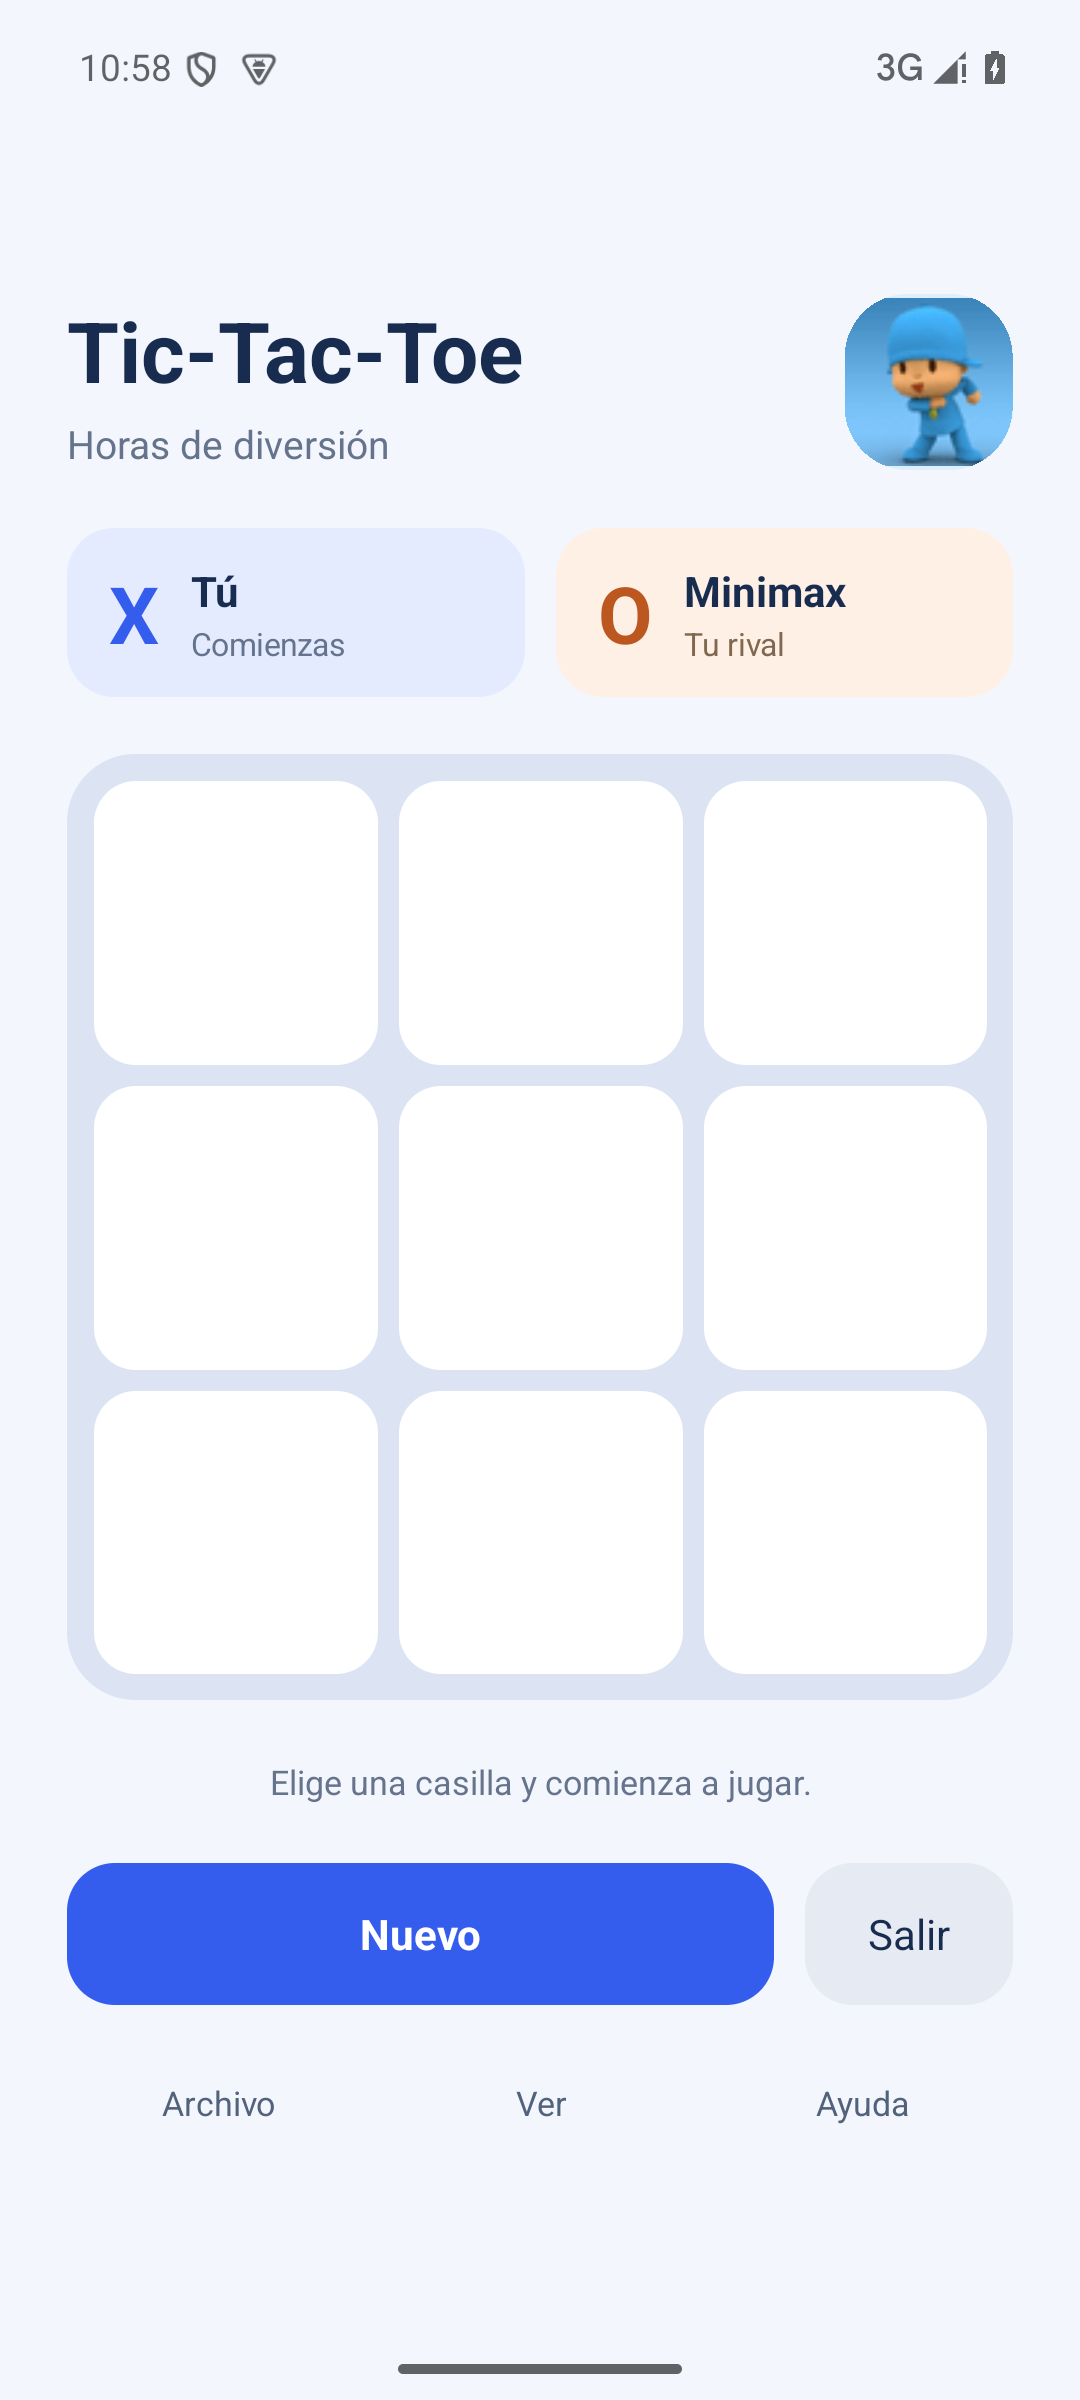
\includegraphics[height=0.78\textheight,keepaspectratio]{figuras/emulador/01_inicio.png}
\caption{Pantalla inicial con el tablero vacío, los símbolos de cada participante y los controles visibles.}\label{fig:emu01}
\end{figure}
\clearpage
\begin{figure}[!htbp]\centering
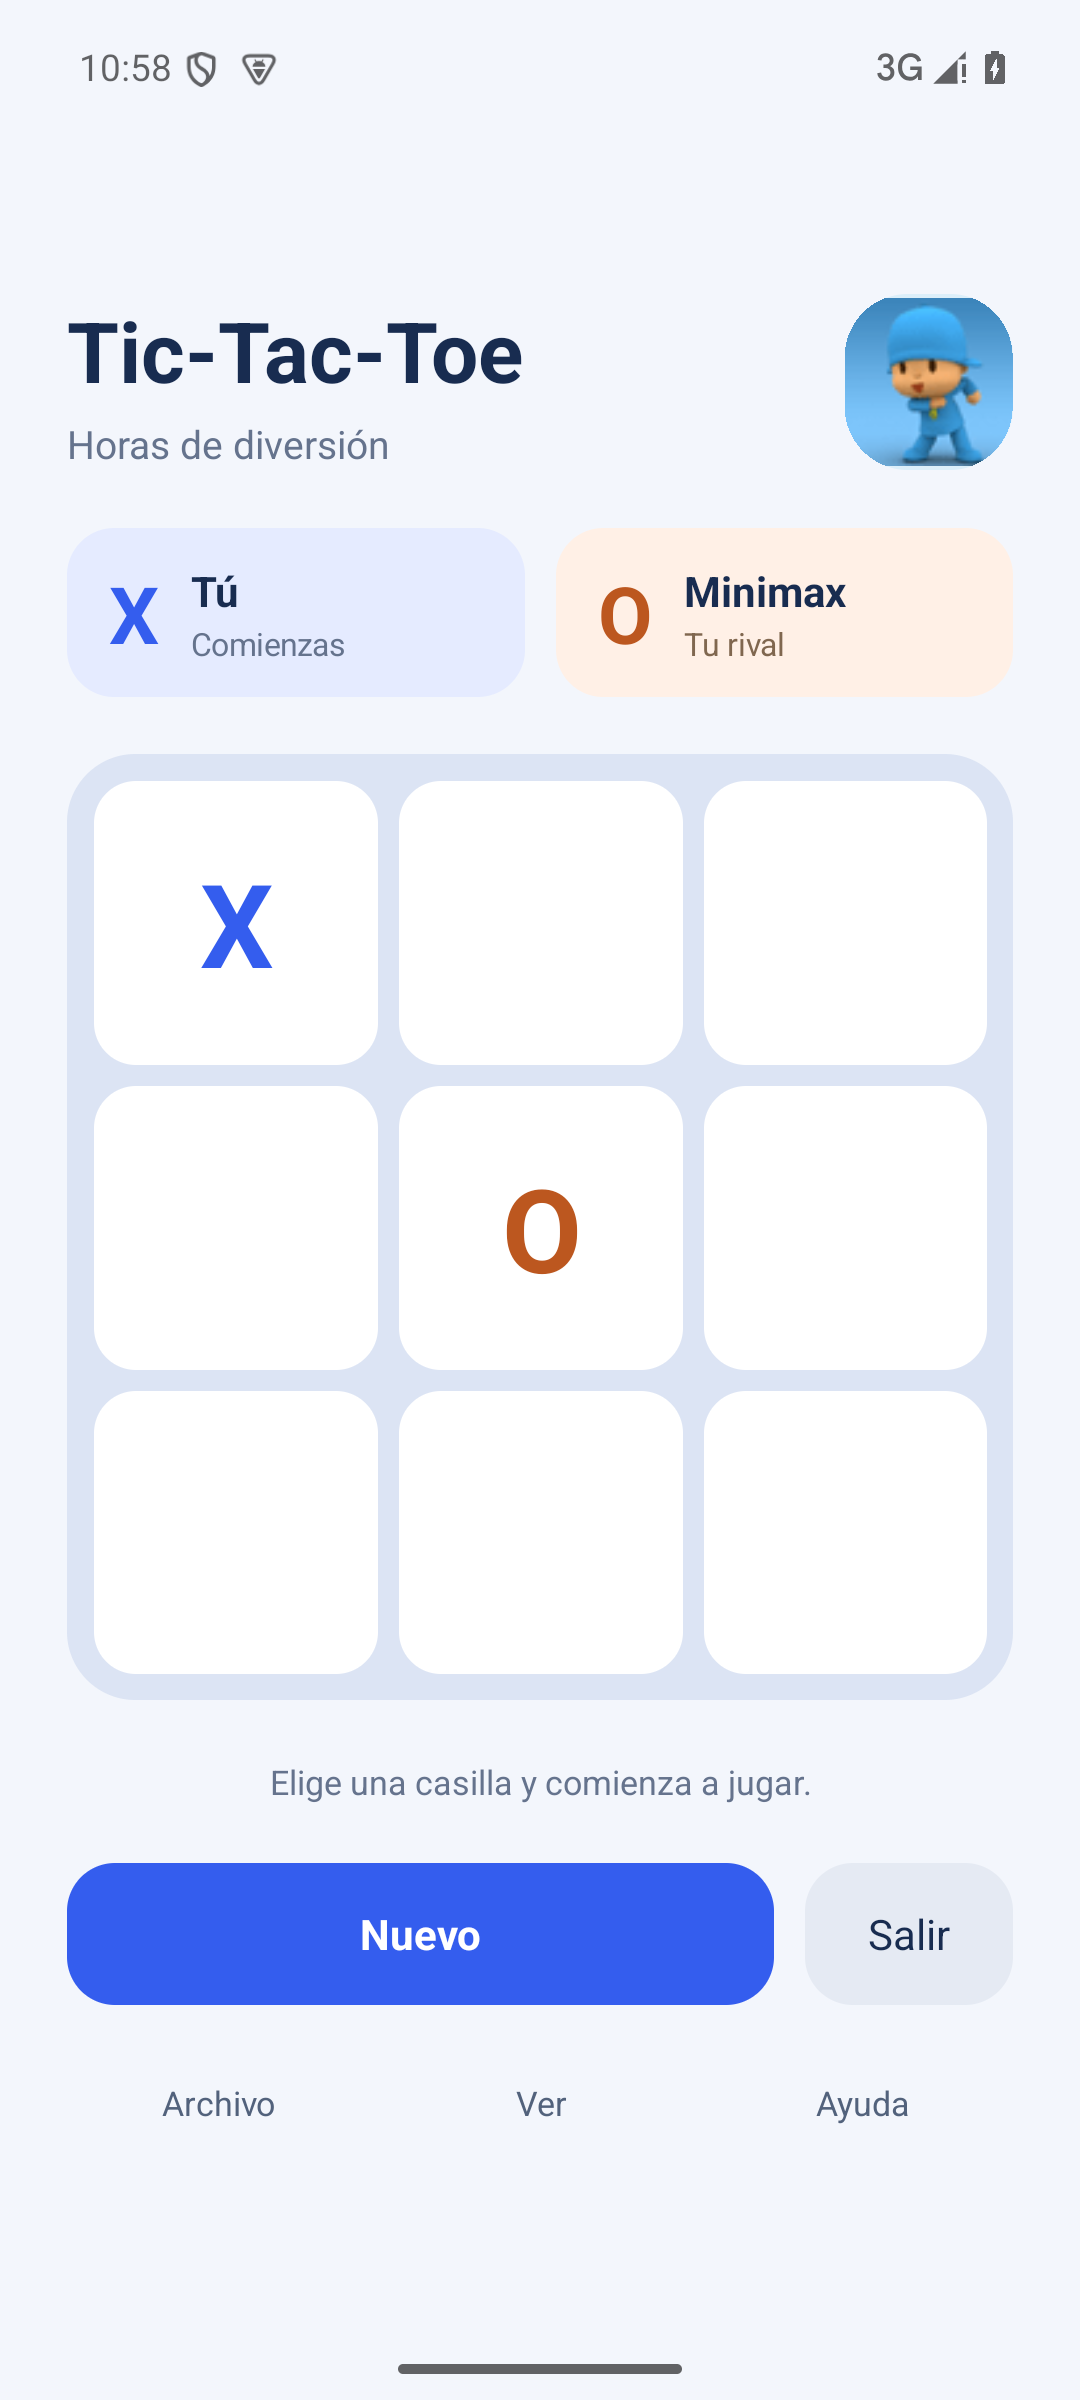
\includegraphics[height=0.78\textheight,keepaspectratio]{figuras/emulador/02_turno_humano_ia.png}
\caption{La persona coloca \texttt{X} y Minimax responde con \texttt{O}.}\label{fig:emu02}
\end{figure}
\clearpage
\begin{figure}[!htbp]\centering
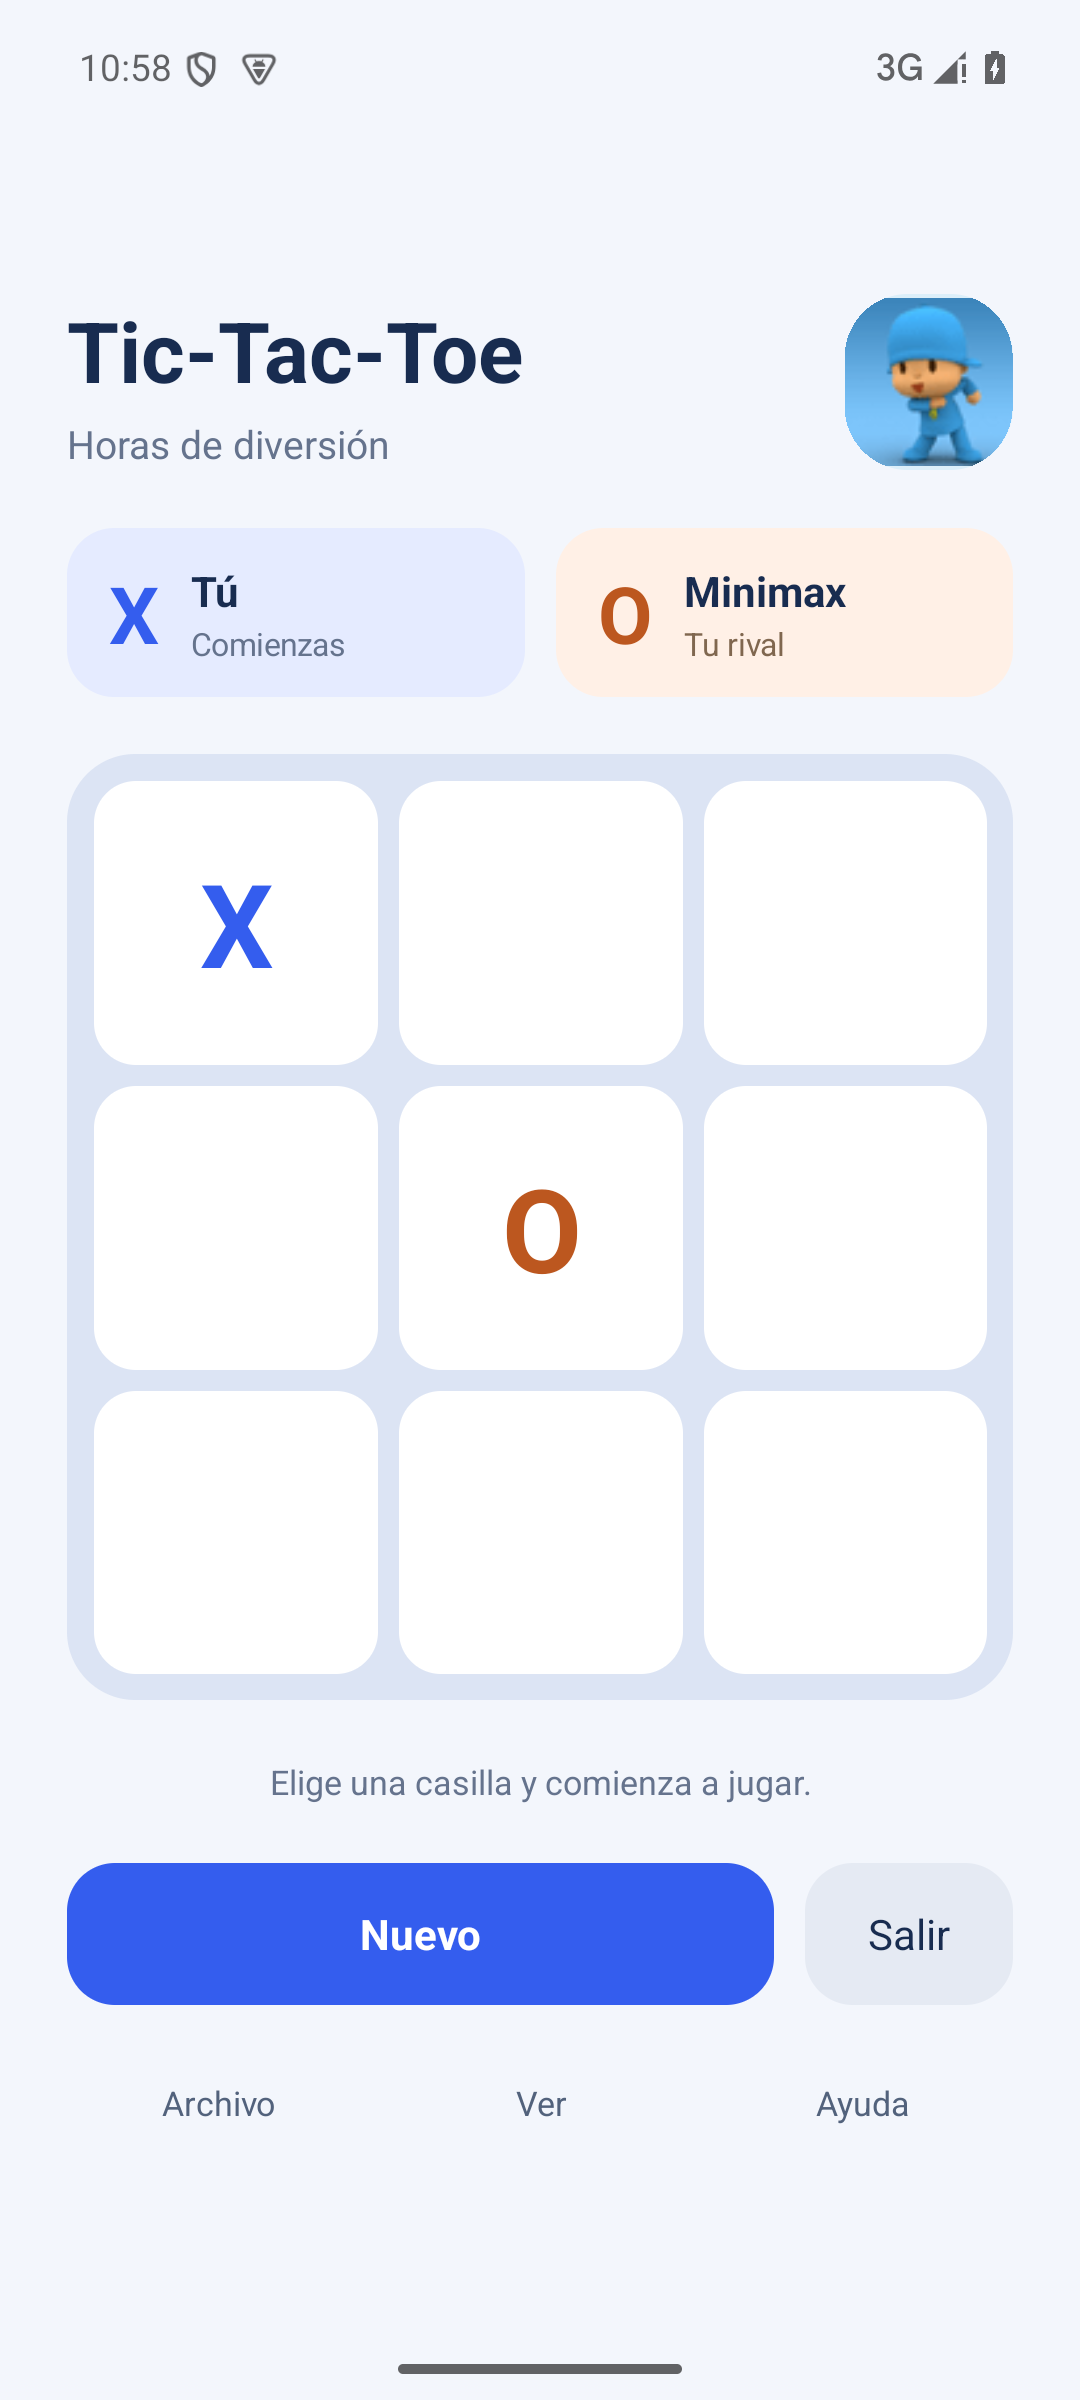
\includegraphics[height=0.78\textheight,keepaspectratio]{figuras/emulador/03_casilla_ocupada.png}
\caption{Verificación registrada para la casilla ocupada; la imagen conserva el mismo hash que la captura 02.}\label{fig:emu03}
\end{figure}
\clearpage
\begin{figure}[!htbp]\centering
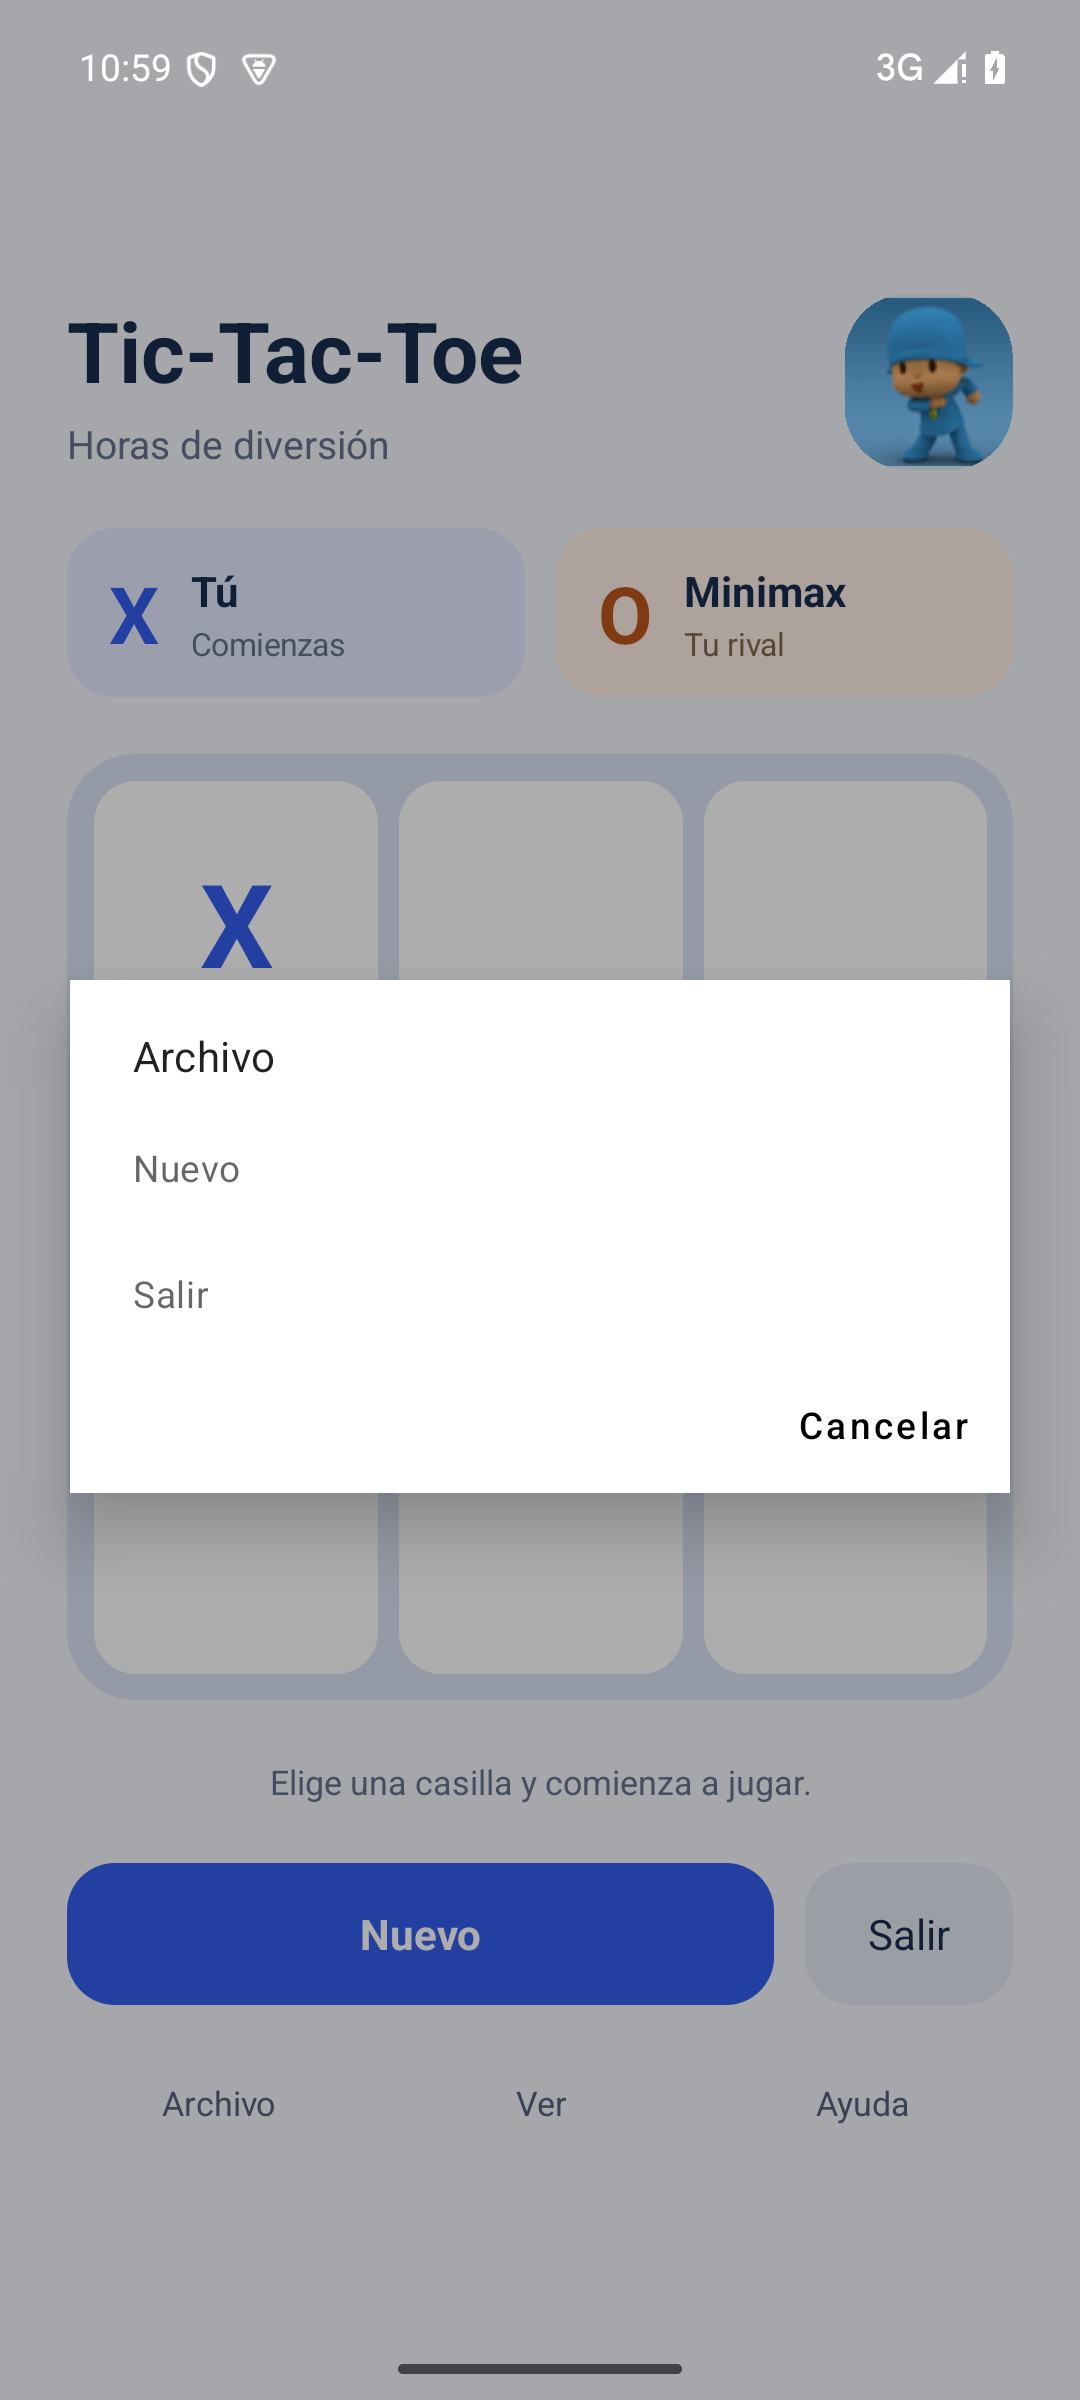
\includegraphics[height=0.78\textheight,keepaspectratio]{figuras/emulador/04_menu_archivo.png}
\caption{Hoja de acciones del menú Archivo. Las opciones no están conectadas a manejadores de acción.}\label{fig:emu04}
\end{figure}
\clearpage
\begin{figure}[!htbp]\centering
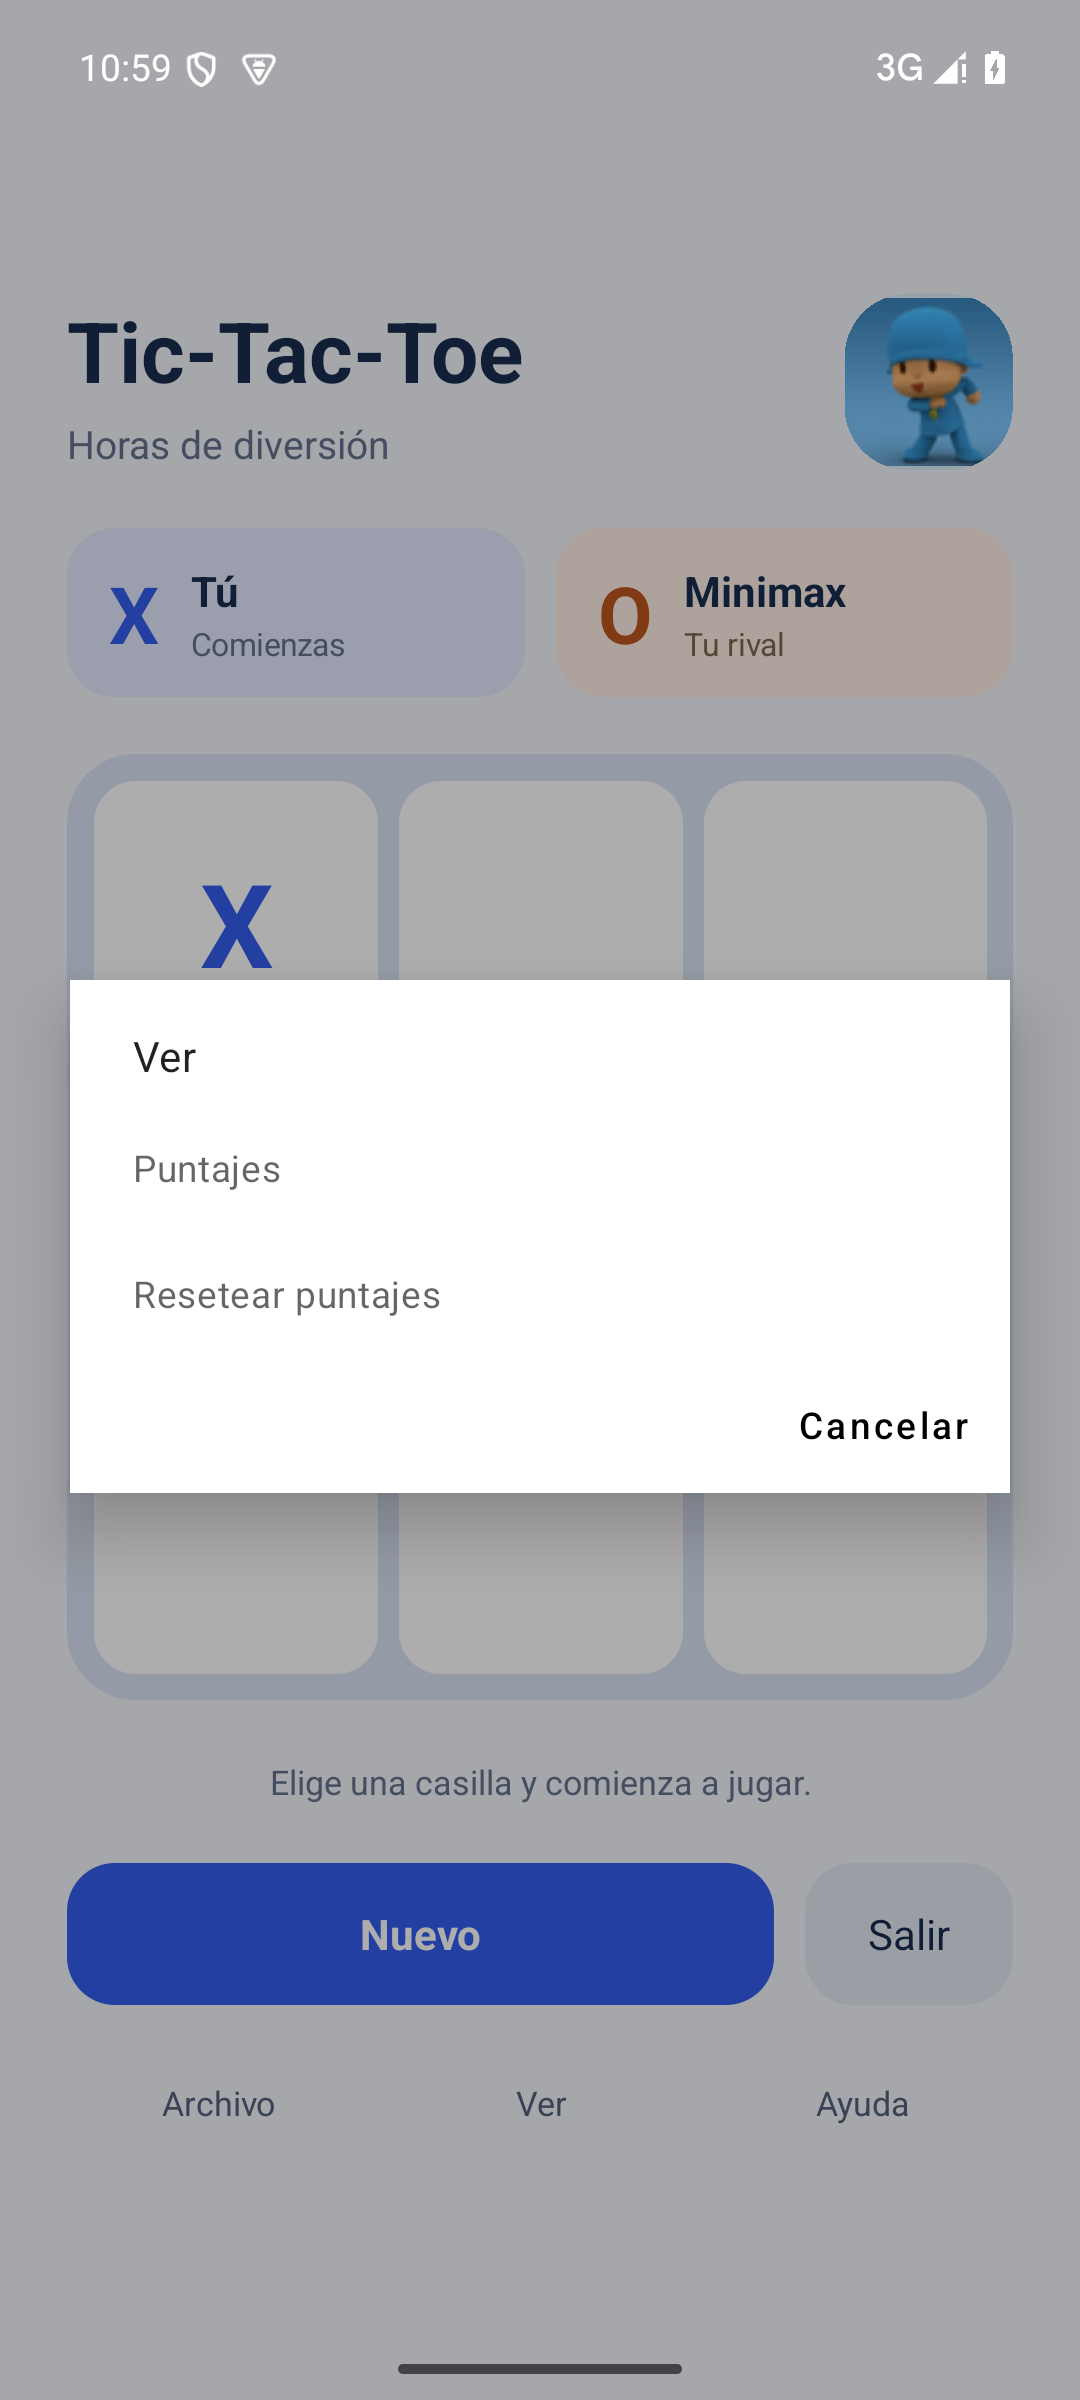
\includegraphics[height=0.78\textheight,keepaspectratio]{figuras/emulador/05_menu_ver.png}
\caption{Hoja de acciones del menú Ver. Puntajes y Resetear puntajes son etiquetas visibles, sin función implementada.}\label{fig:emu05}
\end{figure}
\clearpage
\begin{figure}[!htbp]\centering
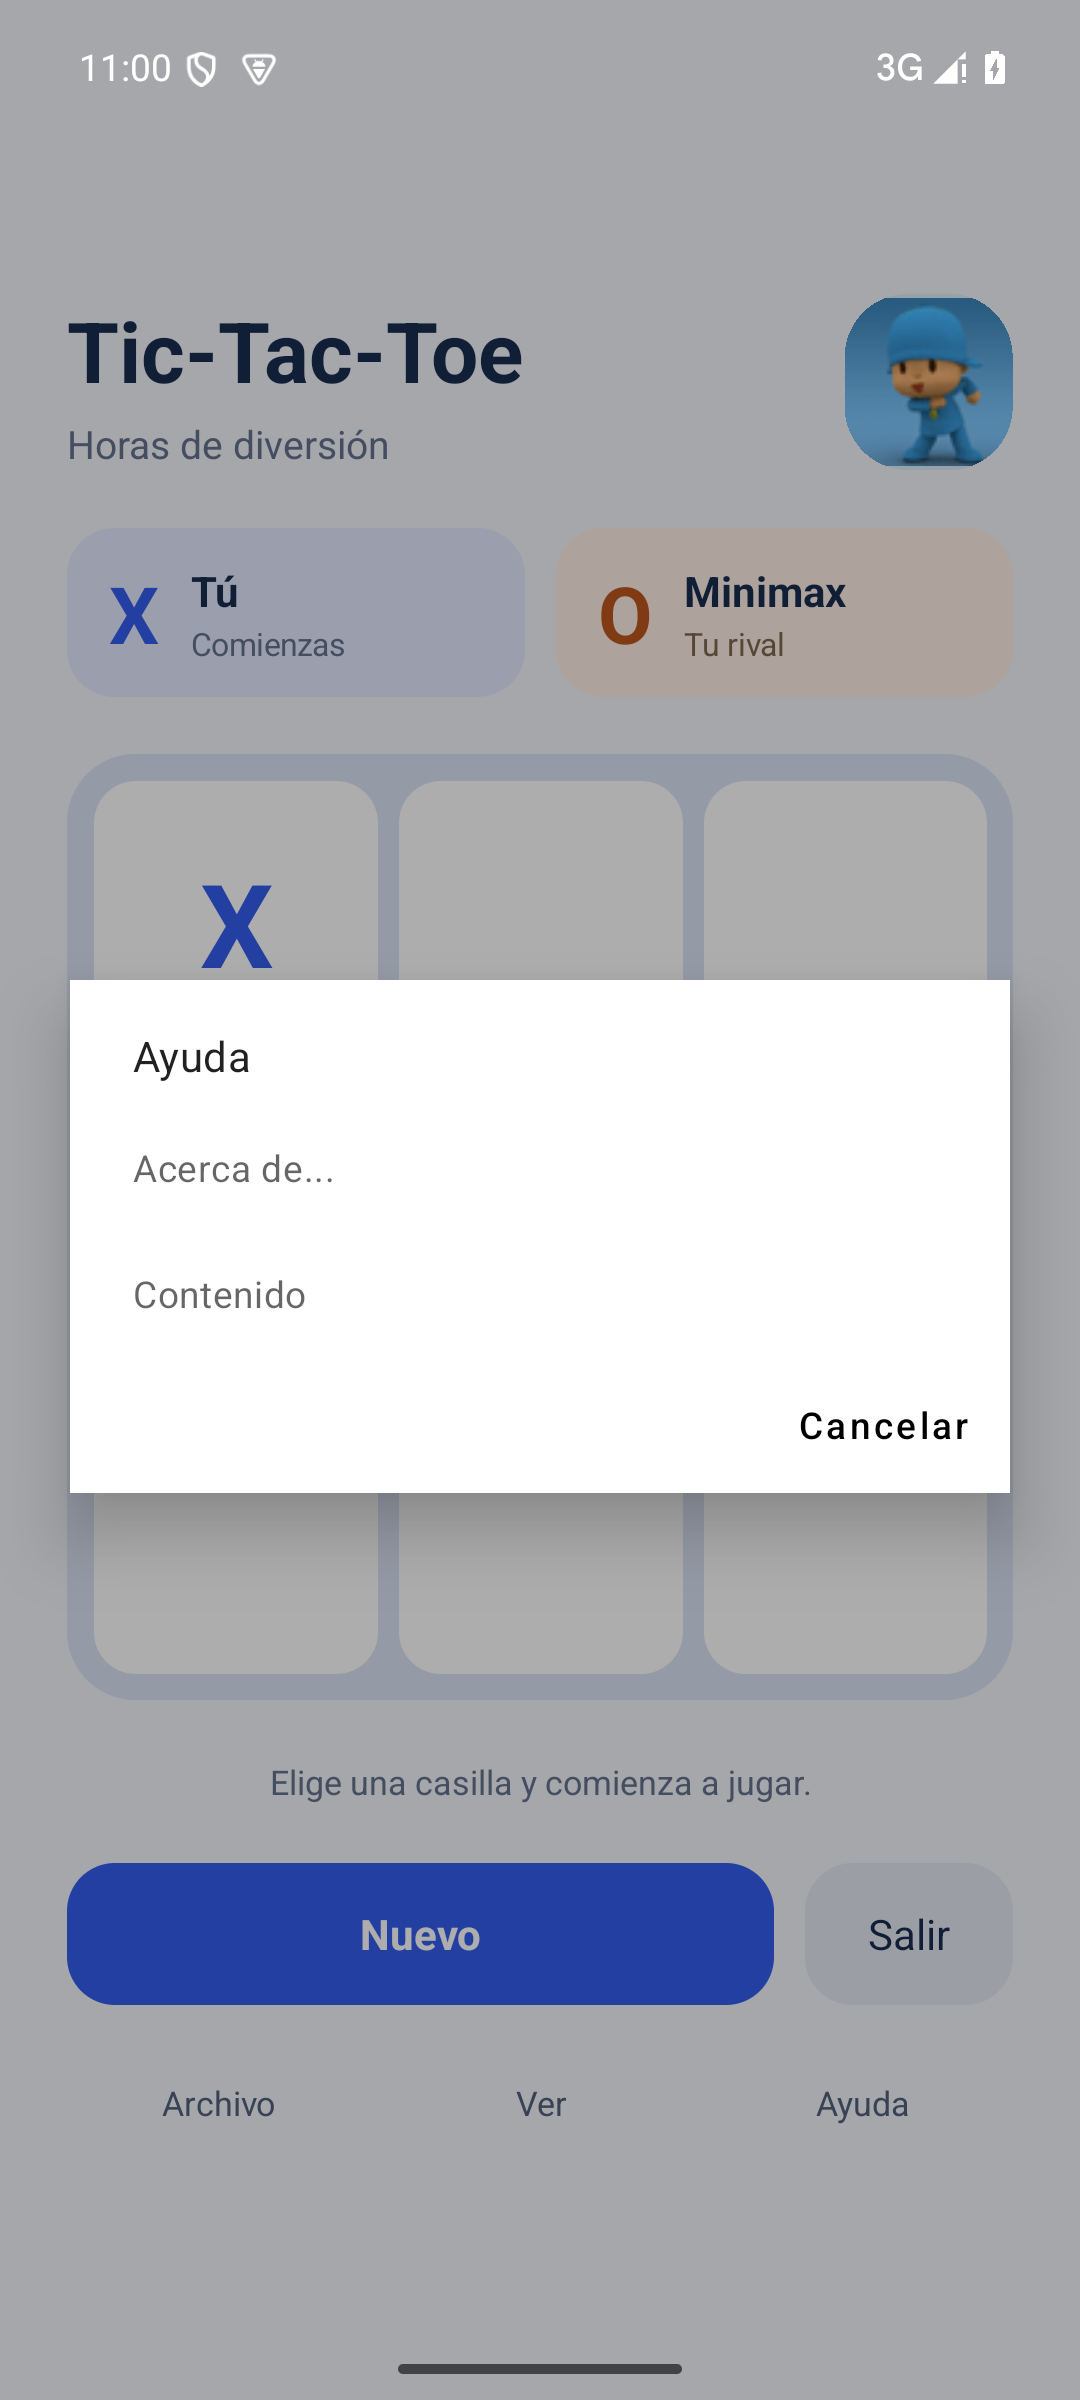
\includegraphics[height=0.78\textheight,keepaspectratio]{figuras/emulador/06_menu_ayuda.png}
\caption{Hoja de acciones del menú Ayuda; las selecciones no abren contenido.}\label{fig:emu06}
\end{figure}
\clearpage
\begin{figure}[!htbp]\centering
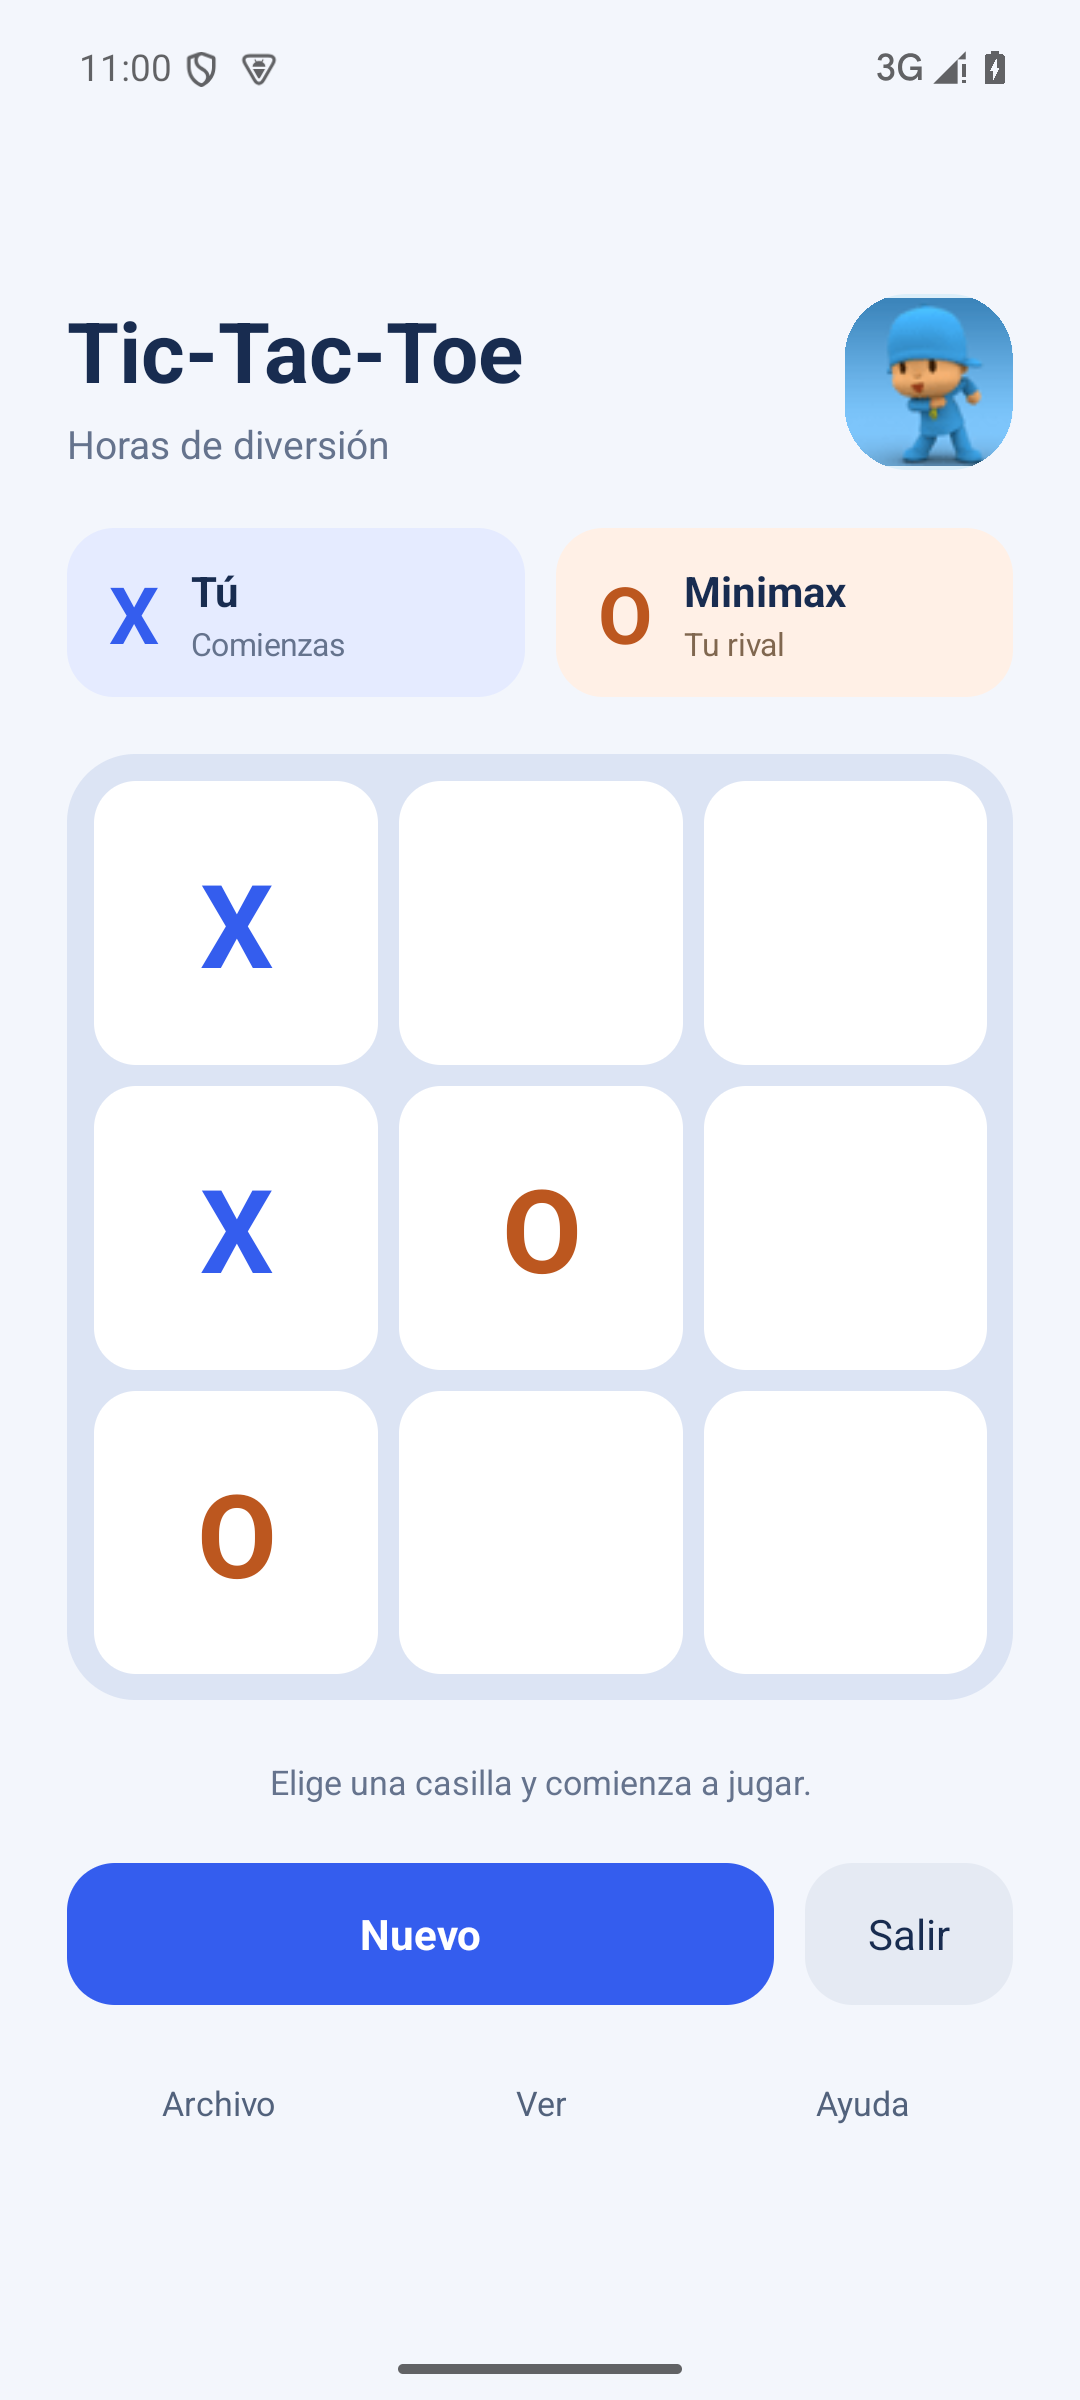
\includegraphics[height=0.78\textheight,keepaspectratio]{figuras/emulador/07_ia_bloquea.png}
\caption{Minimax bloquea la amenaza de victoria de \texttt{X} en la primera columna.}\label{fig:emu07}
\end{figure}
\clearpage
\begin{figure}[!htbp]\centering
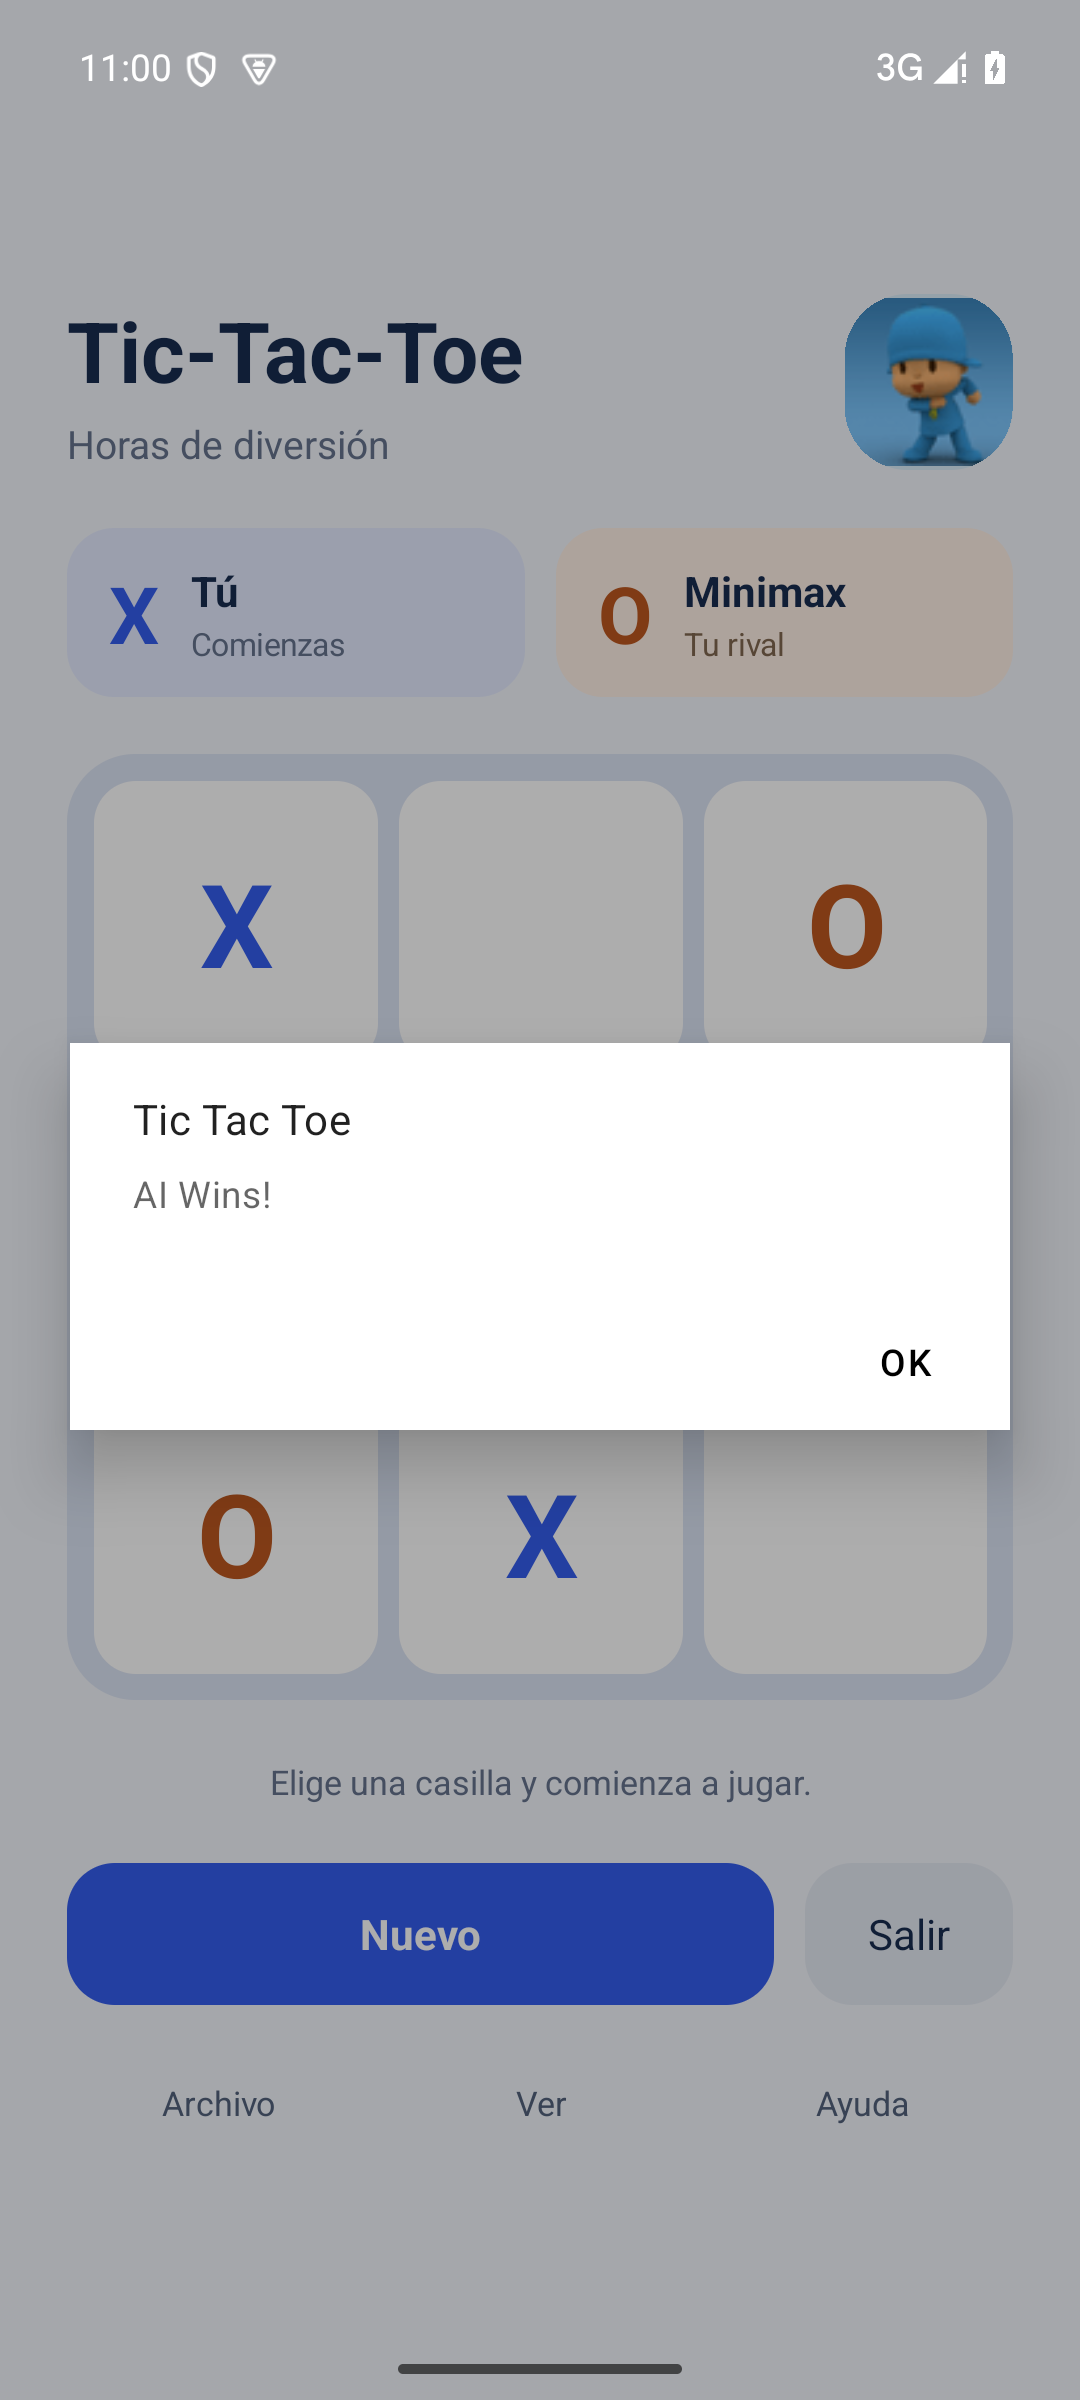
\includegraphics[height=0.78\textheight,keepaspectratio]{figuras/emulador/08_victoria_ia.png}
\caption{Aviso de victoria de la IA registrado en el escenario de prueba.}\label{fig:emu08}
\end{figure}
\clearpage
\begin{figure}[!htbp]\centering
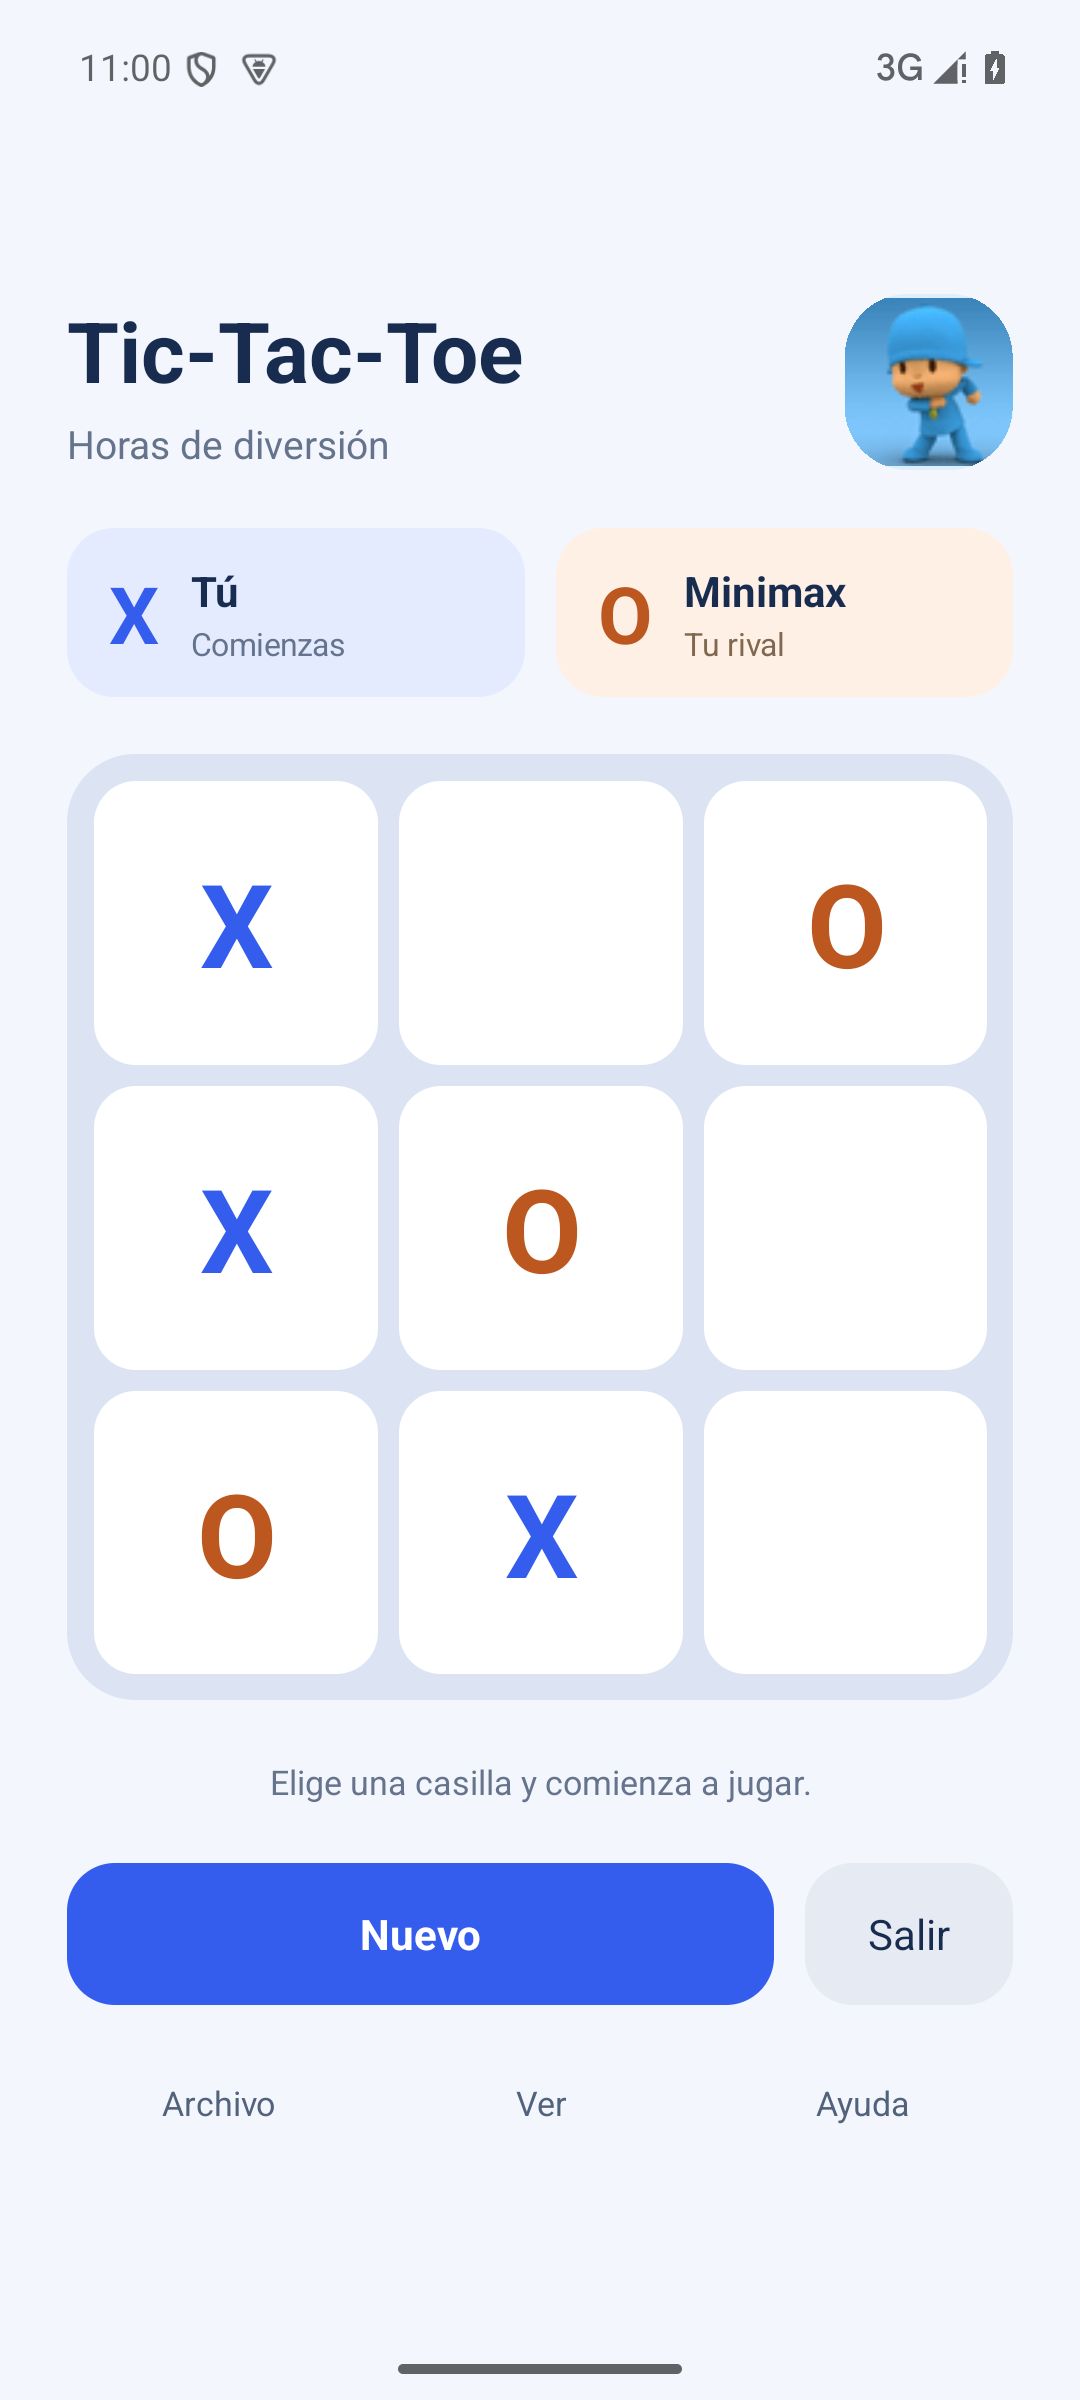
\includegraphics[height=0.78\textheight,keepaspectratio]{figuras/emulador/09_partida_finalizada.png}
\caption{Tablero con victoria diagonal de \texttt{O}; la entrada posterior queda bloqueada.}\label{fig:emu09}
\end{figure}
\clearpage
\begin{figure}[!htbp]\centering
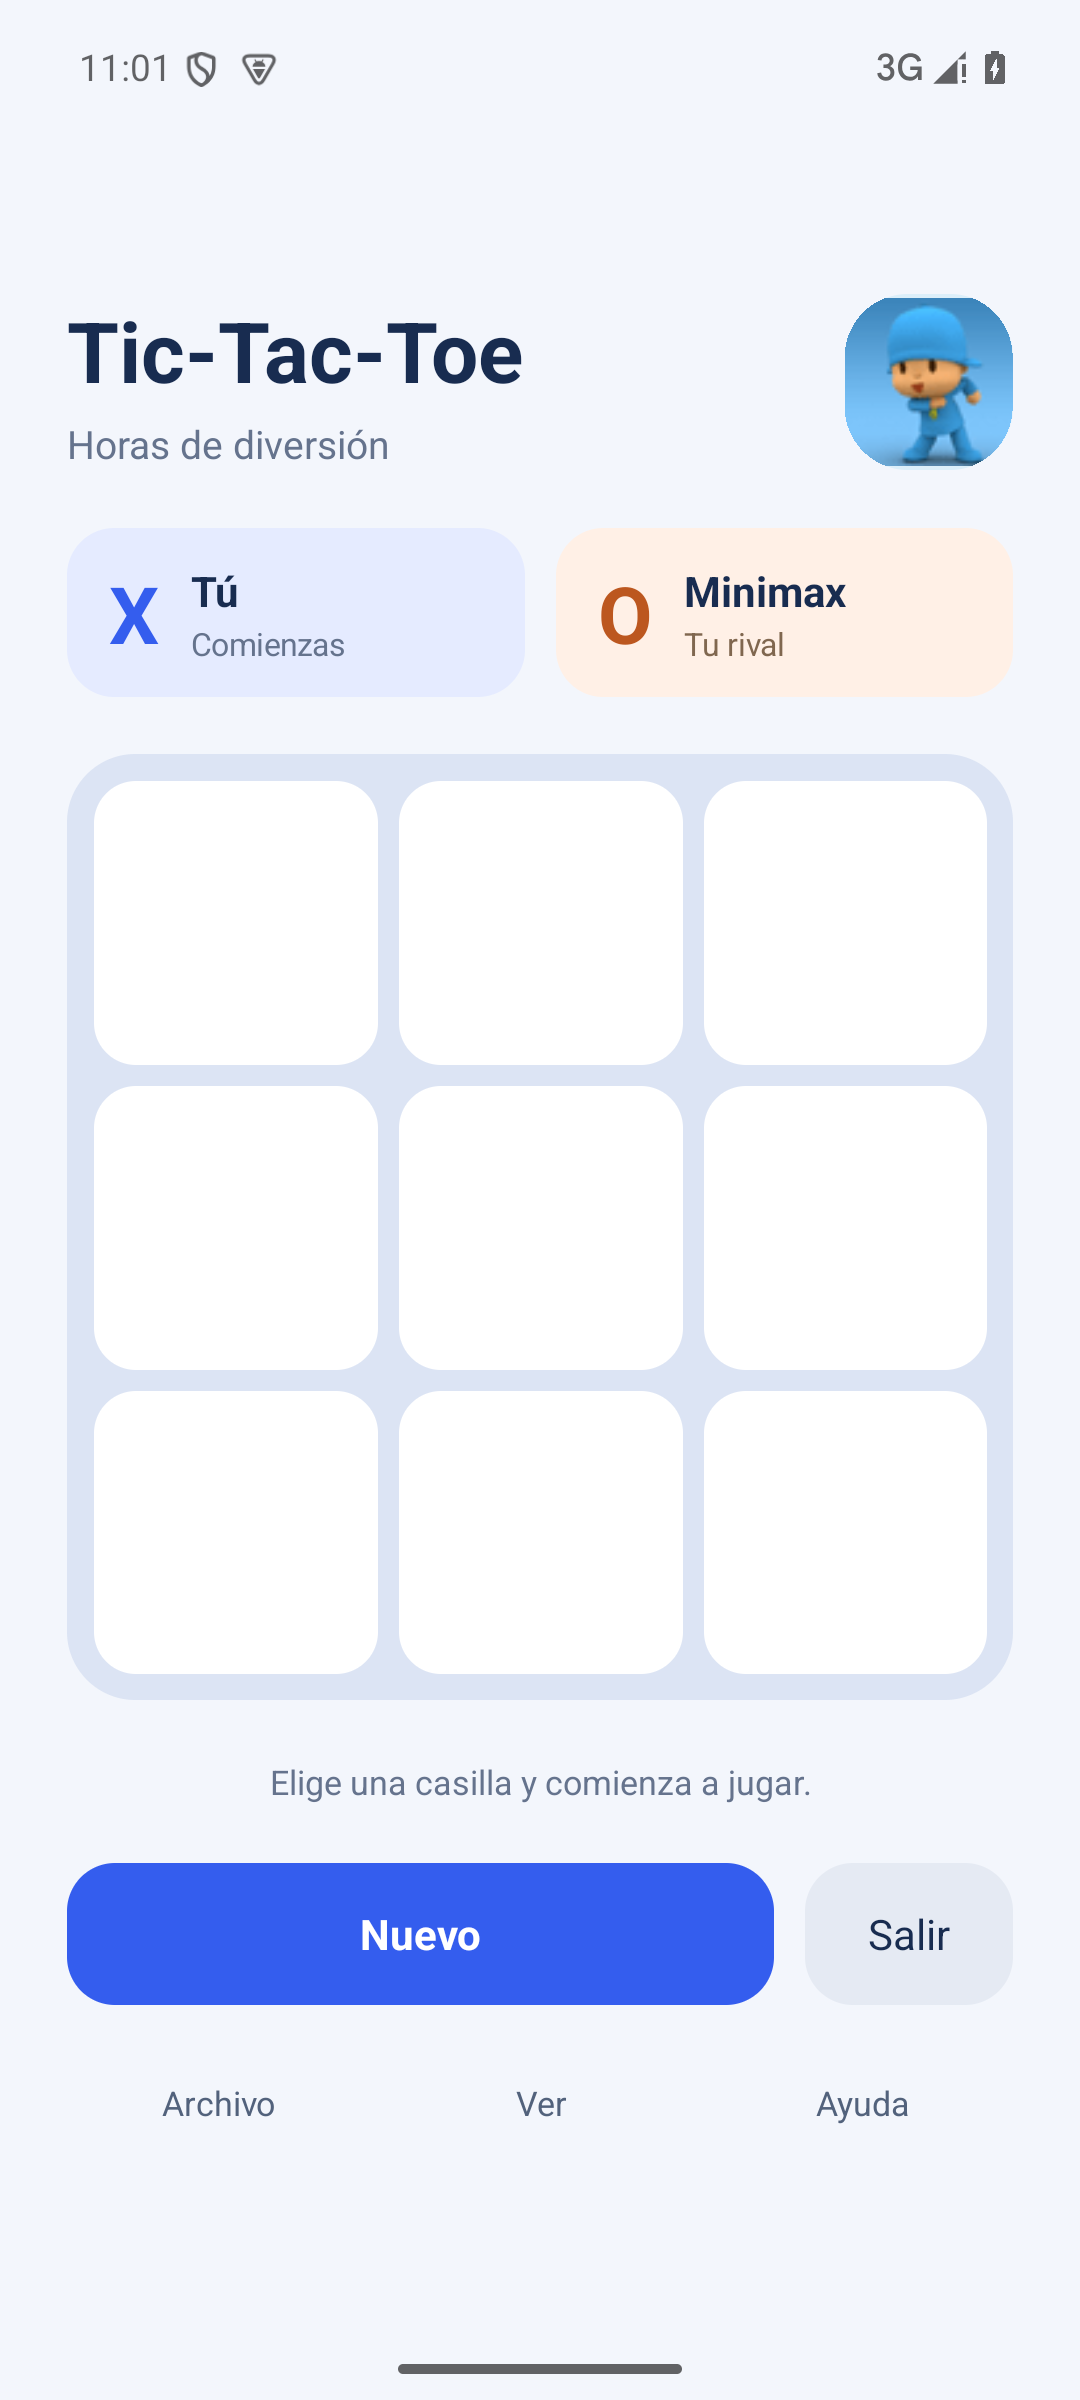
\includegraphics[height=0.78\textheight,keepaspectratio]{figuras/emulador/10_reinicio.png}
\caption{El botón Nuevo limpia la partida y habilita nuevamente las casillas.}\label{fig:emu10}
\end{figure}
\clearpage
\begin{figure}[!htbp]\centering
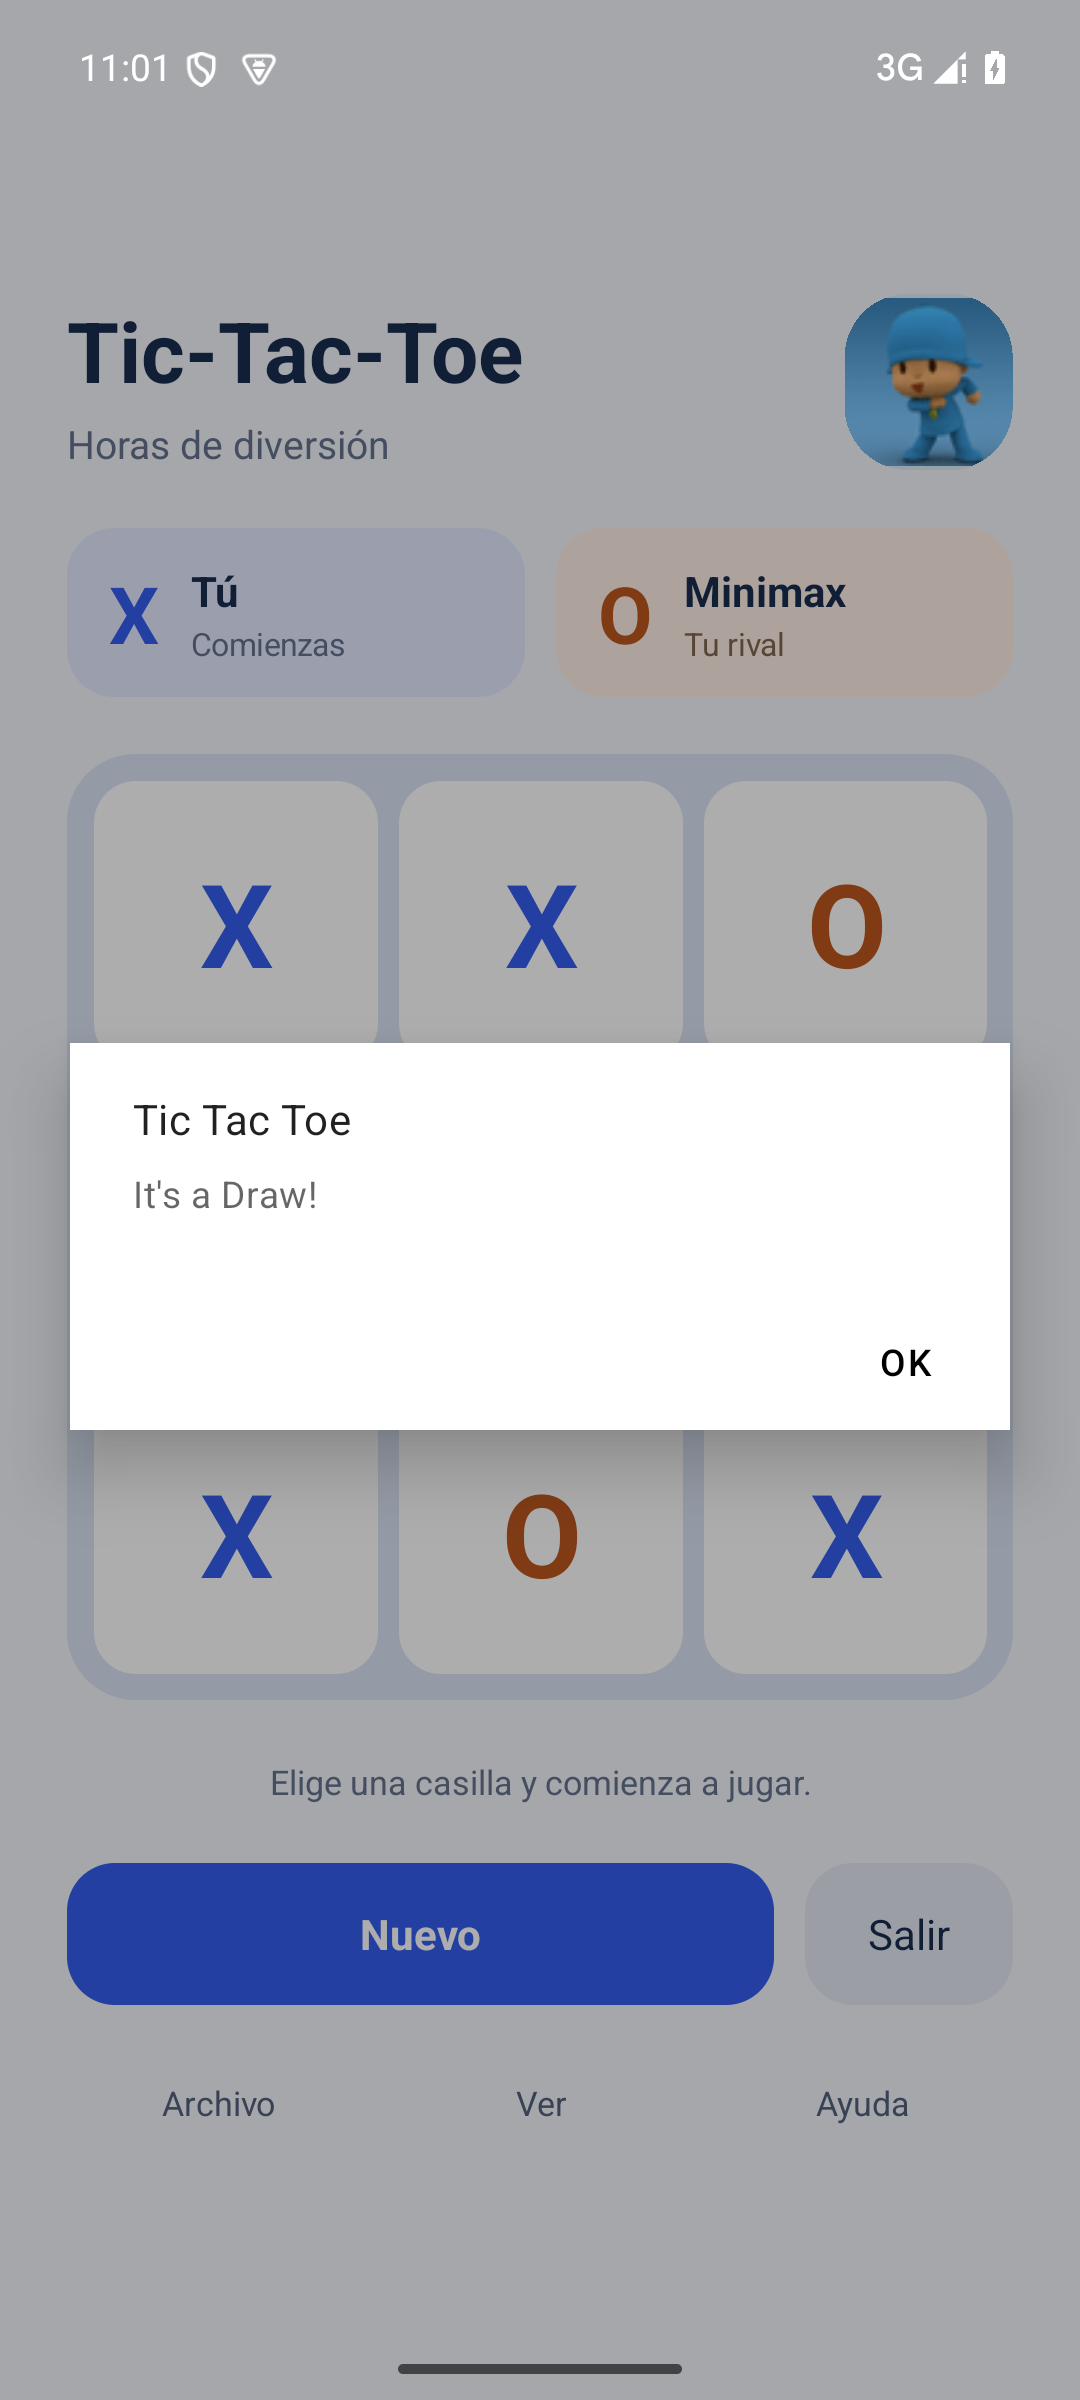
\includegraphics[height=0.78\textheight,keepaspectratio]{figuras/emulador/11_empate_aviso.png}
\caption{Aviso de empate al completar el tablero sin una línea ganadora.}\label{fig:emu11}
\end{figure}
\clearpage
\begin{figure}[!htbp]\centering
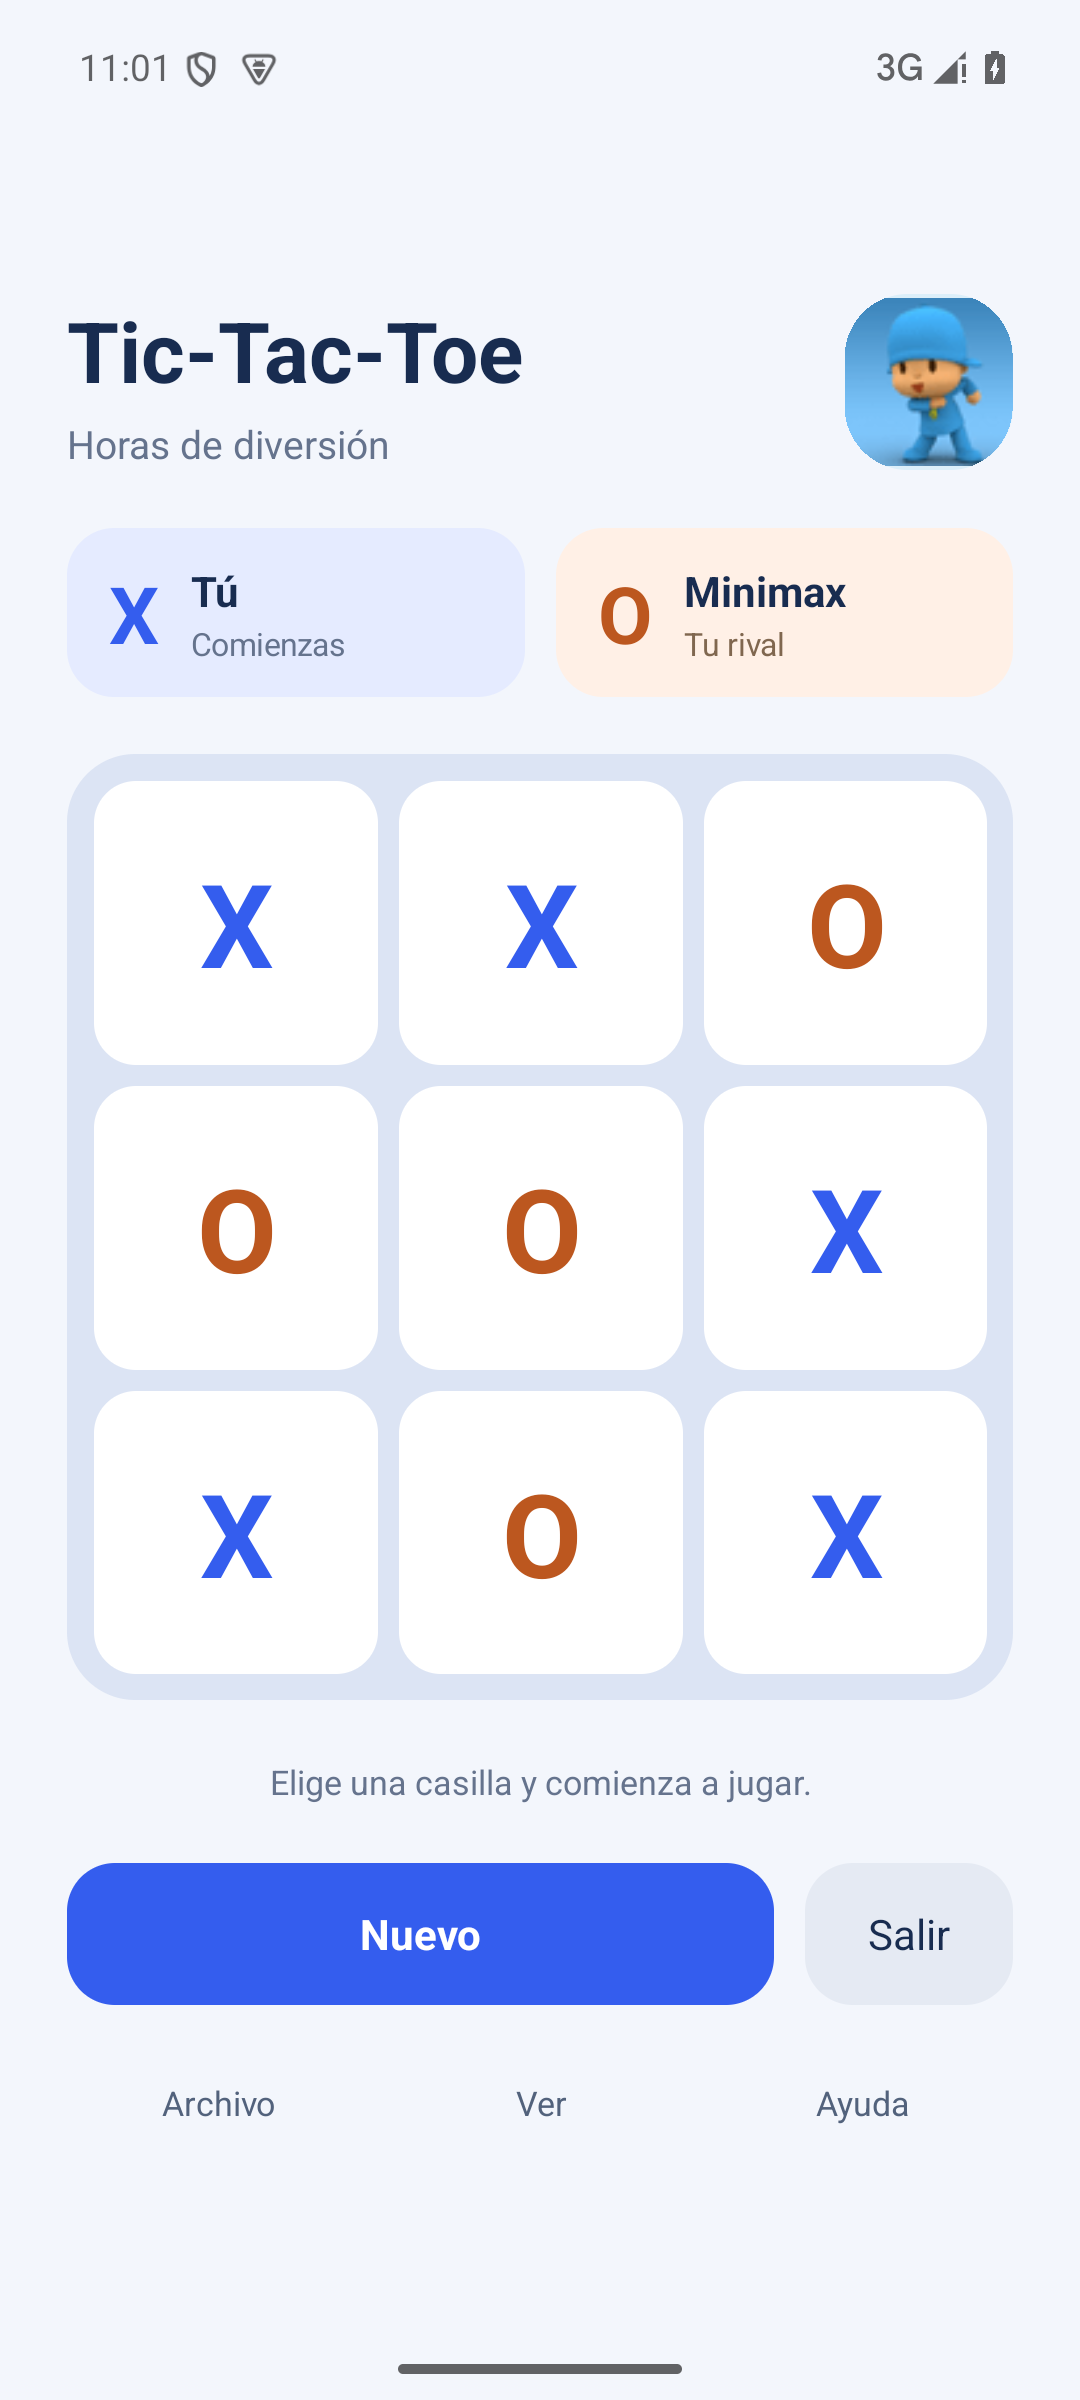
\includegraphics[height=0.78\textheight,keepaspectratio]{figuras/emulador/12_empate_tablero.png}
\caption{Estado final del tablero empatado.}\label{fig:emu12}
\end{figure}
\clearpage
\begin{figure}[!htbp]\centering

\includegraphics[height=0.78\textheight,keepaspectratio]{figuras/emulador/13_salida.png}
\caption{Pantalla de inicio de Android tras usar el botón Salir.}\label{fig:emu13}
\end{figure}
\clearpage
\begin{figure}[!htbp]\centering
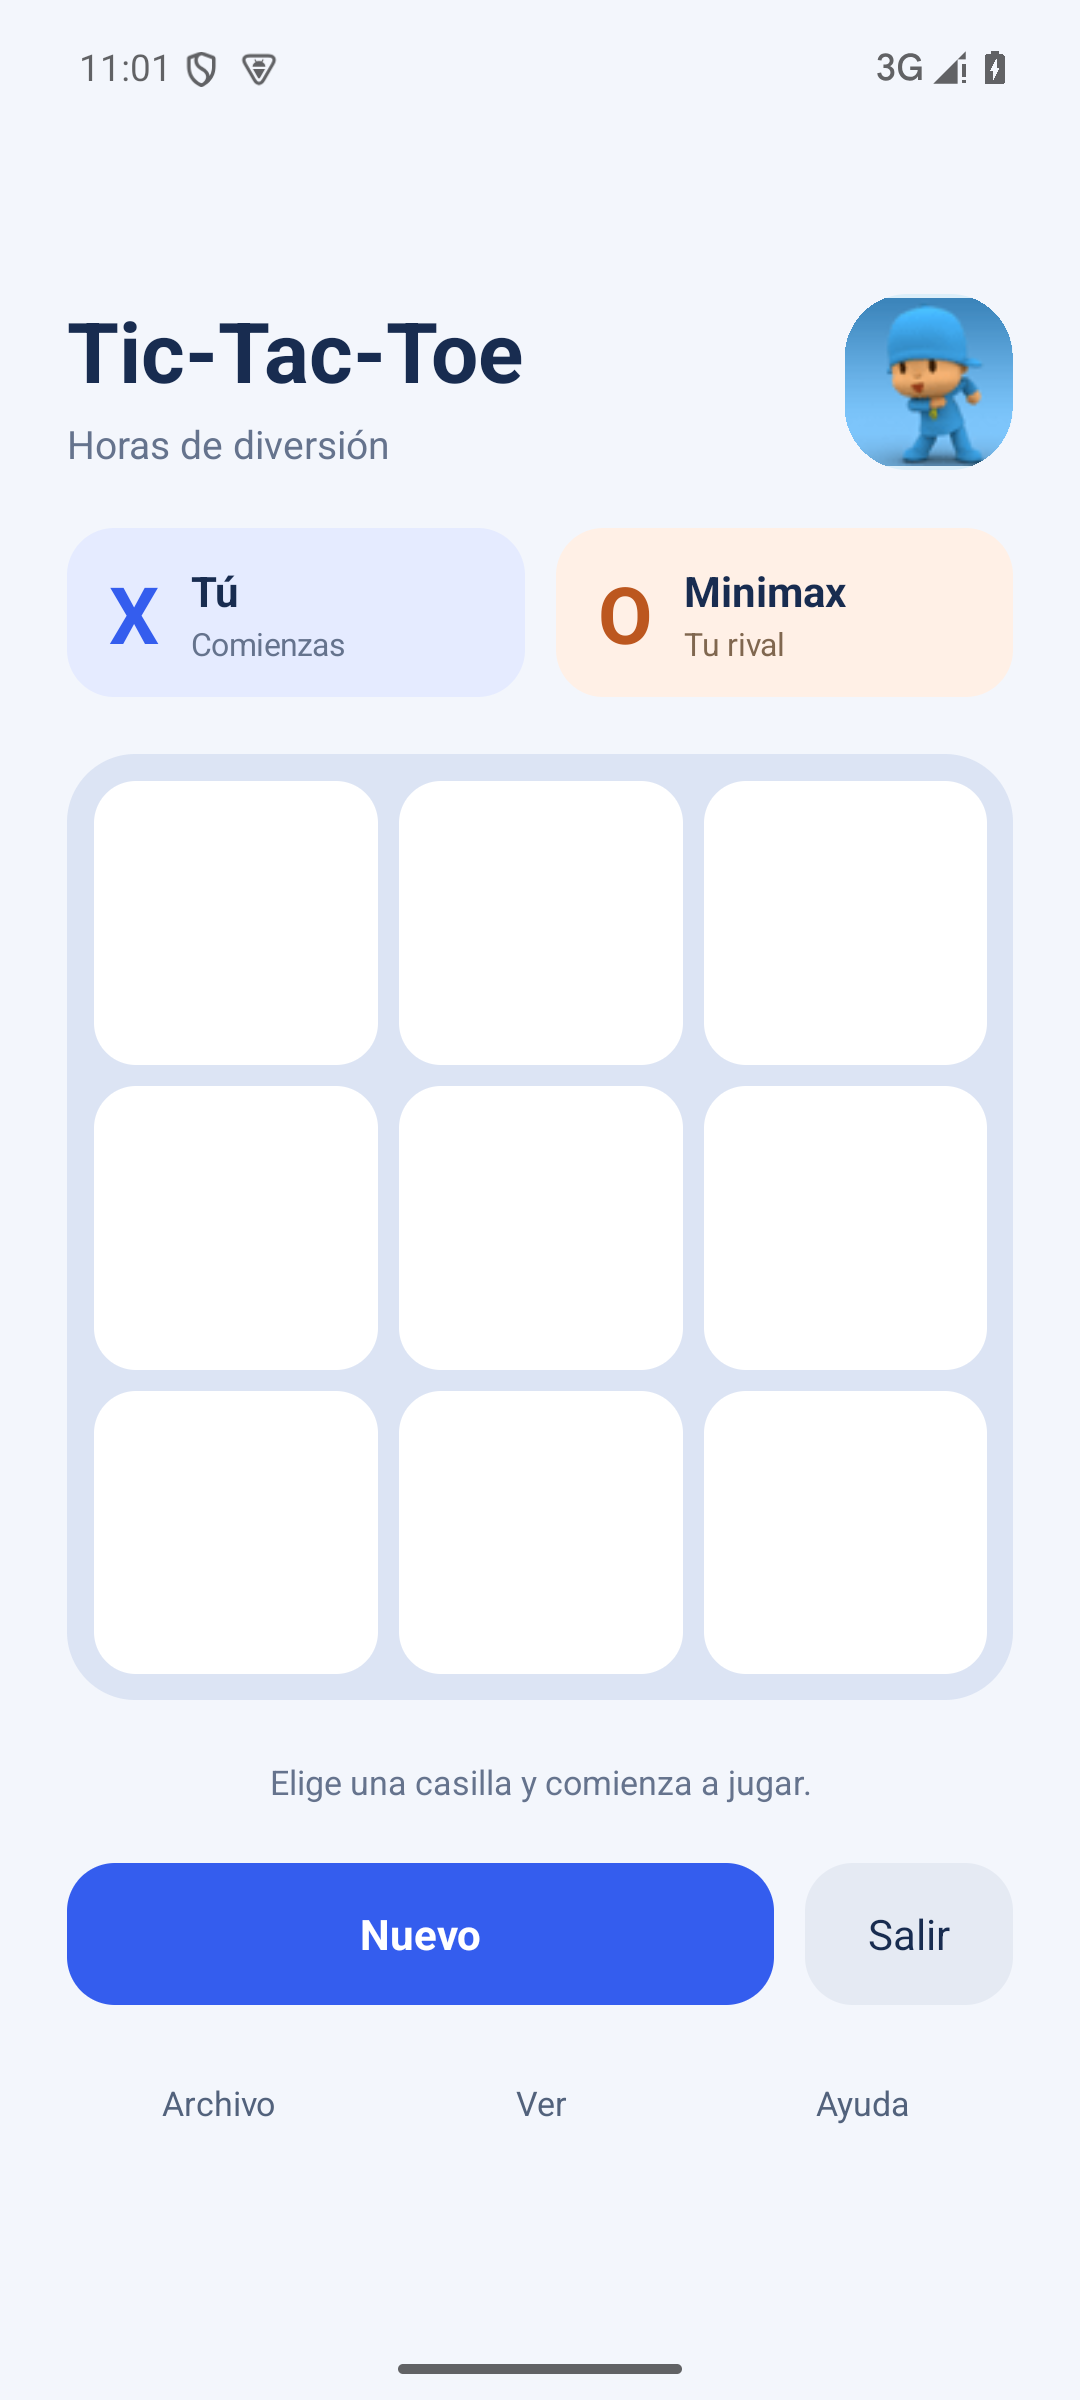
\includegraphics[height=0.78\textheight,keepaspectratio]{figuras/emulador/14_reapertura.png}
\caption{Aplicación reabierta con una partida nueva y tablero vacío.}\label{fig:emu14}
\end{figure}

\end{document}
